%%%%%%%%%%%%%%%%%%%%%%%%%%%%%%%%%%%%%%%%%%%%%%%%%%%%%%%%%%%%%%%%%%%%%%%%%%%%%%%
%                       CARGA DE LA CLASE DE DOCUMENTO                        %
%                                                                             %
% Las opciones admisibles son:                                                %
%      12pt / 11pt            (tamaño del cuerpo de letra; no usar 10pt)      %
%                                                                             %
% catalan/spanish/english     (idioma principal del trabajo)                  %
%                                                                             % 
% french/italian/german...    (si necesitáis usar otro idioma adicional)      %
%                                                                             %
% listoffigures               (El documento incluye un Índice de figuras)     %
% listoftables                (El documento incluye un Índice de tablas)      %
% listofquadres               (El documento incluye un Índice de cuadros)     %
% listofalgorithms            (El documento incluye un Índice de algoritmos)  %
%                                                                             %
%%%%%%%%%%%%%%%%%%%%%%%%%%%%%%%%%%%%%%%%%%%%%%%%%%%%%%%%%%%%%%%%%%%%%%%%%%%%%%%

\documentclass[11pt,english,listoffigures,listoftables]{tfgetsinf}

%%%%%%%%%%%%%%%%%%%%%%%%%%%%%%%%%%%%%%%%%%%%%%%%%%%%%%%%%%%%%%%%%%%%%%%%%%%%%%%
%                     CODIFICACIÓN DEL ARCHIVO FUENTE                         %
%                                                                             %
%    Windows suele usar 'ansinew'                                             %
%    en Linux es posible que sea 'latin1' o 'latin9'                          %
%    Pero lo más recomendable es usar utf8 (unicode 8)                        %
%                                          (si vuestro editor lo permite)     % 
%%%%%%%%%%%%%%%%%%%%%%%%%%%%%%%%%%%%%%%%%%%%%%%%%%%%%%%%%%%%%%%%%%%%%%%%%%%%%%%

\usepackage[utf8]{inputenc} 


%%%%%%%%%%%%%%%%%%%%%%%%%%%%%%%%%%%%%%%%%%%%%%%%%%%%%%%%%%%%%%%%%%%%%%%%%%%%%%%
%                       OTROS PAQUETES Y DEFINICIONES                         %
%                                                                             %
%%%%%%%%%%%%%%%%%%%%%%%%%%%%%%%%%%%%%%%%%%%%%%%%%%%%%%%%%%%%%%%%%%%%%%%%%%%%%%%

\usepackage{glossaries}
\usepackage{textcomp}
\usepackage{booktabs}
\usepackage{float}
\usepackage{enumitem}
\usepackage{graphicx}
\usepackage{subcaption}
\usepackage{tabularx}
\usepackage{algorithm}
\usepackage{algpseudocode}
\usepackage{pgfplots}
\pgfplotsset{compat=1.18}
\usepgfplotslibrary{groupplots}
\usetikzlibrary{positioning,arrows.meta,calc,babel,automata}

% Listings para código
\usepackage{listings}
\lstset{
  basicstyle=\ttfamily\small,
  frame=single,
  breaklines=true,
  postbreak=\mbox{\textcolor{gray}{$\hookrightarrow$}\space},
  columns=fullflexible,
  keepspaces=true,
  numbers=none
}

% Bibliografía
\usepackage[backend=biber,style=numeric,sorting=none]{biblatex}
\addbibresource{bibliografia.bib}

% Hyperref siempre al final
\usepackage{hyperref}
\hypersetup{
  colorlinks=true,
  linkcolor=black,
  urlcolor=cyan,
  citecolor=black
}
%%%%%%%%%%%%%%%%%%%%%%%%%%%%%%%%%%%%%%%%%%%%%%%%%%%%%%%%%%%%%%%%%%%%%%%%%%%%%%%
%                        DADES DEL TREBALL                                    %
%                                                                             %
% titol, alumne, tutor i curs academic                                        %
%%%%%%%%%%%%%%%%%%%%%%%%%%%%%%%%%%%%%%%%%%%%%%%%%%%%%%%%%%%%%%%%%%%%%%%%%%%%%%%

\title{FARM: A Formal Approach to Reward Machine Generation in Reinforcement Learning}
\author{Miquel Gómez}
\tutor{Eva Onaindía De La Rivaherrera}
\curs{2026-2027}

%%%%%%%%%%%%%%%%%%%%%%%%%%%%%%%%%%%%%%%%%%%%%%%%%%%%%%%%%%%%%%%%%%%%%%%%%%%%%%%
%                     PARAULES CLAU/PALABRAS CLAVE/KEY WORDS                  %
%                                                                             %
% Independentment de la llengua del treball, s'hi han d'incloure              %
% les paraules clau i el resum en els tres idiomes                            %
%%%%%%%%%%%%%%%%%%%%%%%%%%%%%%%%%%%%%%%%%%%%%%%%%%%%%%%%%%%%%%%%%%%%%%%%%%%%%%%

\keywords{Aprenentatge per reforç; Màquina de recompensa; Lògica temporal lineal; Especificació de tasques en llenguatge natural} % Paraules clau
         {Aprendizaje por refuerzo; Máquina de recompensa; Lógica temporal lineal; Especificación de tareas en lenguaje natural} % Palabras clave
         {Reinforcement Learning; Reward Machine; Linear Temporal Logic; Natural Language Task Specification} % Key words

%%%%%%%%%%%%%%%%%%%%%%%%%%%%%%%%%%%%%%%%%%%%%%%%%%%%%%%%%%%%%%%%%%%%%%%%%%%%%%%
%                              INICI DEL DOCUMENT                             %
%%%%%%%%%%%%%%%%%%%%%%%%%%%%%%%%%%%%%%%%%%%%%%%%%%%%%%%%%%%%%%%%%%%%%%%%%%%%%%%

\begin{document}

%%%%%%%%%%%%%%%%%%%%%%%%%%%%%%%%%%%%%%%%%%%%%%%%%%%%%%%%%%%%%%%%%%%%%%%%%%%%%%%
%              RESUMS DEL TFG EN VALENCIA, CASTELLA I ANGLES                  %
%%%%%%%%%%%%%%%%%%%%%%%%%%%%%%%%%%%%%%%%%%%%%%%%%%%%%%%%%%%%%%%%%%%%%%%%%%%%%%%

\begin{abstract}
La construcció automàtica de màquines de recompensa (\foreign{english}{Reward Machines}, RM) en l'aprenentatge per reforç s'ha explorat recentment amb grans models fundacionals, que generen RM directament a partir de descripcions de tasques en llenguatge natural. Tot i ser prometedors, aquests mètodes no ofereixen garanties formals i depenen d'avaluacions qualitatives, fetes per persones, de la correcció de les RM. En aquest treball proposem FARM (\foreign{english}{A Formal Approach to Reward Machine Generation in Reinforcement Learning}), una cadena de processament basada en la lògica temporal lineal (LTL) per a generar RM: les tasques en llenguatge natural es tradueixen primer a fórmules LTL, que després es compilen en màquines de recompensa amb eines de la teoria d'autòmats. Aquest enfocament produeix RM que, per construcció, estan alineades amb l'especificació temporal desitjada. Introduïm un conjunt de mètriques estructurals i de comportament per a avaluar la qualitat de les RM, i avaluem el rendiment de l'aprenentatge per reforç en termes de taxa d'èxit i d'eficiència mostral en la resolució de tasques. En un banc de proves de tasques amb estructura temporal, el nostre mètode basat en LTL produeix RM més fidels a l'especificació de la tasca i condueix a un aprenentatge més ràpid i fiable que les RM generades per un enfocament de l'estat de l'art basat en models fundacionals. Aquests resultats suggereixen que la síntesi formal de RM guiada per la lògica ofereix una alternativa robusta i interpretable als mètodes de generació de recompenses purament neuronals.
\end{abstract}

\begin{abstract}[spanish]
La construcción automática de máquinas de recompensa (\foreign{english}{Reward Machines}, RM) en el aprendizaje por refuerzo se ha explorado recientemente con grandes modelos fundacionales, que generan RM directamente a partir de descripciones de tareas en lenguaje natural. Aunque prometedores, estos métodos carecen de garantías formales y dependen de evaluaciones cualitativas, realizadas por personas, de la corrección de las RM. En este trabajo proponemos FARM (\foreign{english}{A Formal Approach to Reward Machine Generation in Reinforcement Learning}), una cadena de procesamiento basada en la lógica temporal lineal (LTL) para generar RM: las tareas en lenguaje natural se traducen primero a fórmulas LTL, que después se compilan en máquinas de recompensa con herramientas de la teoría de autómatas. Este enfoque produce RM que, por construcción, están alineadas con la especificación temporal deseada. Introducimos un conjunto de métricas estructurales y de comportamiento para evaluar la calidad de las RM, y evaluamos el rendimiento del aprendizaje por refuerzo en términos de tasa de éxito y eficiencia muestral en la resolución de tareas. En un banco de pruebas de tareas con estructura temporal, nuestro método basado en LTL produce RM más fieles a la especificación de la tarea y conduce a un aprendizaje más rápido y fiable que las RM generadas por un enfoque del estado del arte basado en modelos fundacionales. Estos resultados sugieren que la síntesis formal de RM guiada por la lógica ofrece una alternativa robusta e interpretable a los métodos de generación de recompensas puramente neuronales.
\end{abstract}

% Keeps the English heading with its text (the Valencian and Spanish abstracts fill page iii).
\newpage
\begin{abstract}[english]
The automated construction of Reward Machines (RMs) in Reinforcement Learning has recently been explored using large foundation models, which generate RMs directly from natural language task descriptions. While promising, these methods lack formal guarantees and rely on qualitative, human-evaluated assessments of RM correctness. In this work, we propose FARM: A Formal Approach to Reward Machine Generation in Reinforcement Learning. A pipeline based on Linear Temporal Logic (LTL) for RM generation: natural language tasks are first translated into LTL formulas, which are then compiled into Reward Machines using automata-theoretic tools. This approach produces RMs that, by construction, are aligned with the desired temporal specification. We introduce a set of structural and behavioral metrics to evaluate RM quality, and assess reinforcement learning performance in terms of success rate and sample efficiency in task resolution. On a benchmark of temporally structured tasks, our LTL-based method produces RMs more faithful to the task specification and leads to faster, more reliable learning compared to RMs generated by a state-of-the-art foundation model approach. These results suggest that logic-guided formal RM synthesis offers a robust and interpretable alternative to purely neural reward generation methods.
\end{abstract}

\chapter{Acknowledgements}
% TODO

\chapter{Glossary}
% TODO

%%%%%%%%%%%%%%%%%%%%%%%%%%%%%%%%%%%%%%%%%%%%%%%%%%%%%%%%%%%%%%%%%%%%%%%%%%%%%%%
%                              CONTINGUT DEL TREBALL                          %
%%%%%%%%%%%%%%%%%%%%%%%%%%%%%%%%%%%%%%%%%%%%%%%%%%%%%%%%%%%%%%%%%%%%%%%%%%%%%%%

\mainmatter

%%%%%%%%%%%%%%%%%%%%%%%%%%%%%%%%%%%%%%%%%%%%%%%%%%%%%%%%%%%%%%%%%%%%%%%%%%%%%%%
%                                 INTRODUCTION                                %
%%%%%%%%%%%%%%%%%%%%%%%%%%%%%%%%%%%%%%%%%%%%%%%%%%%%%%%%%%%%%%%%%%%%%%%%%%%%%%%

\chapter{Introduction}
\label{chap:introduction}
\section{Motivation}
\section{Objectives}
\section{Expected impact}
\section{Structure of the paper}
\section{Scope and limits of the study}
% Scope facts for the final text (no prose yet):
% - FARM takes ARM-FM's setting and improves only the generation of the Reward Machine (RM). The
%   labelling functions and the state descriptions and embeddings follow ARM-FM and are not
%   evaluated. The comparison with ARM-FM is isolated to RM generation.
% - The ARM-FM paper releases no code. A public repository of the first author (not referenced in
%   the paper, no licence) holds prompts, machines and labelling code for four MiniGrid tasks only.
%   The baseline is rebuilt from the paper and that material; the authors did not answer the
%   contact attempts; the results may differ from theirs.
% - FARM generates with small models (generator deepseek-v4.1-flash and critic glm-5.3-flash, as
%   resolved from the environment on 2026-10-29; reasoning level none and three attempts are the
%   defaults of app/src/config/config.py). ARM-FM used GPT-4o.
% - LTLf over finite traces; the eight Declare templates of IBM nl2ltl; no RM minimisation
%   (future work); prompt ablations are planned.

%%%%%%%%%%%%%%%%%%%%%%%%%%%%%%%%%%%%%%%%%%%%%%%%%%%%%%%%%%%%%%%%%%%%%%%%%%%%%%%
%                               STATE OF THE ART                              %
%%%%%%%%%%%%%%%%%%%%%%%%%%%%%%%%%%%%%%%%%%%%%%%%%%%%%%%%%%%%%%%%%%%%%%%%%%%%%%%

\chapter{State of the art}
\label{chap:sota}
\section{Related work}
\subsection{Reward Machines}
\label{sec:sota-rm}
In reinforcement learning (RL), an agent learns to act in a Markov decision process (MDP) by maximising the reward it receives \cite{sutton2018reinforcement}. Most methods treat the reward function as a black box: the agent observes the number returned after each step and nothing about how it is computed \cite{icarte2022reward}. A person writes that function by hand, and a hand-programmed reward can be exploited. Randl{\o}v and Alstr{\o}m \cite{randlov1998learning} shaped the reward of a bicycle-riding agent and observed it circling instead of reaching its destination. Amodei et al.~\cite{amodei2016concrete} and Skalse et al.~\cite{skalse2022defining} describe this failure as reward hacking: the agent obtains a high reward without doing what the designer intended.

Sparse rewards pose a second problem. When the reward arrives only on completing a long task, the agent receives almost no signal while it learns. Reward shaping adds intermediate reward to guide it. Ng et al.~\cite{ng1999policy} prove that shaping with the difference of a potential function over states, $\gamma\Phi(s') - \Phi(s)$, leaves the optimal policy unchanged, and that no other form of shaping gives this guarantee in general.

Reward Machines (RMs) address both problems by exposing the structure of the reward to the learner. Toro Icarte et al.~\cite{toroicarte2018using} introduced them at ICML 2018 and gave a fuller account in the Journal of Artificial Intelligence Research (JAIR) \cite{icarte2022reward}. This thesis follows the JAIR article for the formalisation, counterfactual learning and reward shaping.

An RM is a finite-state machine, written $\langle U, u_0, F, \delta_u, \delta_r\rangle$ in the JAIR formulation. $U$ is a finite set of states, $u_0 \in U$ the initial state and $F$ the set of terminal states. The transition function $\delta_u$ takes the current state and the set of propositions that hold and returns the next state. The reward function $\delta_r$ assigns to each state a reward function over environment transitions. The ICML formulation attaches the reward to the pair of states of a transition instead, which is the convention of the RM text format used in this thesis.

Propositions come from outside the machine. A labelling function $L$ maps each environment transition to the set of propositions that hold in it, for example ``the agent holds the key''. At every step the machine reads that set and moves. The agent learns in the product of the MDP and the RM, whose states pair an environment state with an RM state; in the product the reward is Markovian even when the task is not.

Exposing the structure enables dedicated learning methods. Q-learning for RMs (QRM) \cite{toroicarte2018using} decomposes the machine and learns, off-policy, one sub-policy per RM state in parallel. The JAIR article adds counterfactual reasoning for RMs (CRM), which reuses each experience to update every RM state; a hierarchical method (HRM); and automated reward shaping. The shaping potential is the negative optimal value of the RM state, $\Phi(s,u) = -v^{*}(u)$, computed by value iteration on the machine (Section~4.4 of the article, restricted to simple RMs).

RMs have two costs. Someone has to design the machine, and the authors note that RMs do not remove the difficulty of designing reward functions, although they may make temporally extended behaviours easier to specify \cite{icarte2022reward}. The labelling function is also assumed to exist and to be correct: learning RMs from experience, one of the open problems listed in the article, needs a correct labelling function. Both costs motivate generating RMs automatically.

\subsection{ARM-FM}
\label{sec:sota-armfm}
ARM-FM (Automated Reward Machines via Foundation Models), by Creus Castanyer et al.~\cite{creus2026armfm} and published at ICLR 2026, replaces the hand-built RM with one generated by a foundation model (FM) from a natural-language task description. The output is a Language-Aligned Reward Machine (LARM), made of three parts: an RM, the Python code of its labelling functions, and a natural-language description of each RM state. A text embedding of the description of the current state is given to the policy together with the environment observation, so that the policy knows which sub-goal is active. In this thesis ARM-FM is the method and LARM its output.

The RM is produced by a generator model and reviewed by a critic model over several rounds of self-improvement. A human may optionally approve the result or give corrective feedback. The generator prompt asks for the machine as plain text in a fixed format. The critic prompt asks, among other checks, that regressions are penalised and that no unintentional loops exist, and the critic answers either \texttt{NO CHANGES NEEDED} or \texttt{CHANGES REQUIRED} \cite[pp.~26--27]{creus2026armfm}. The paper uses GPT-4o to generate all LARM components, except for the 1\,000 XLand-MiniGrid LARMs, which come from several open-source models.

The evaluation covers four environments: MiniGrid (DoorKey and the harder UnlockToUnlock, BlockedUnlockPickup and KeyCorridor), Craftium (a Minecraft-based environment where the agent mines a diamond after gathering wood, stone and iron), Meta-World manipulation tasks, and XLand-MiniGrid. On DoorKey the agent trained with the LARM outperforms DQN with ICM, ReAct and plain DQN; on the three harder MiniGrid tasks it is the only agent that solves all of them; on Craftium it learns where an agent without the LARM makes no progress. On XLand-MiniGrid a single policy trains on ten tasks at once and solves unseen combinations of known tasks without fine-tuning.

Listing~\ref{lst:armfm-doorkey} reproduces the DoorKey machine printed in the appendix of the paper. Listing~\ref{lst:farm-example1} shows the machine FARM generates for the first running example of Chapter~\ref{chap:farm}.

\begin{lstlisting}[caption={The DoorKey Reward Machine printed by ARM-FM (page 30 of the paper).},label={lst:armfm-doorkey}]
REWARD_MACHINE:
STATES: u0, u1, u2, u3
INITIAL_STATE: u0
TRANSITION_FUNCTION:
(u0, has_key) -> u1
(u0, else) -> u0
(u1, is_door_in_env_open) -> u2
(u1, not_has_key) -> u0
(u1, else) -> u1
(u2, at_goal) -> u3
(u2, else) -> u2
(u3, else) -> u3
REWARD_FUNCTION:
(u0, has_key, u1) -> 0.2
(u1, is_door_in_env_open, u2) -> 0.3
(u1, not_has_key, u0) -> -0.2
(u2, at_goal, u3) -> 1.0
\end{lstlisting}

\lstinputlisting[caption={The Reward Machine FARM generates for the first running example.},label={lst:farm-example1}]{images/farm/rm-ex1.txt}

The format of FARM differs from that of ARM-FM in five points.
\begin{itemize}
    \item There are no \texttt{else} self-loops. A state with no matching transition stays where it is and pays the default reward.
    \item The states with a special role are listed explicitly: \texttt{FINAL\_STATES}, \texttt{REJECTING\_STATES} and \texttt{ACCEPTING\_STATES}.
    \item A single event expression combines propositions with \texttt{!} and \texttt{\&}, such as \texttt{has\_key \& !door\_open}, instead of a separate predicate such as \texttt{not\_has\_key}.
    \item \texttt{DEFAULT\_REWARD}, \texttt{HARD\_FAILED\_REWARD} and \texttt{SOFT\_FAILED\_REWARD} fix the reward of a transition without an entry and the charge for a failed promise.
    \item \texttt{PENDING\_PROMISES} lists, for each state, the hard and soft obligations still open.
\end{itemize}
Appendix~\ref{app:running} lists the machine of a task made only of rules, where the last two points apply.

\subsection{Linear Temporal Logic}
\label{sec:sota-ltl}
Linear Temporal Logic (LTL) is a logic for stating properties of sequences of states, called traces. Pnueli \cite{pnueli1977temporal} proposed it to reason about programs. It is a language rather than a catalogue of patterns: a formula is built from propositions, Boolean connectives and four temporal operators.
\begin{itemize}
    \item $\mathrm{X}\,\varphi$ (next): $\varphi$ holds at the next step.
    \item $\mathrm{F}\,\varphi$ (eventually): $\varphi$ holds at the current step or at a later one.
    \item $\mathrm{G}\,\varphi$ (always): $\varphi$ holds at every step from the current one on.
    \item $\varphi\ \mathrm{U}\ \psi$ (until): $\psi$ holds at some step from the current one on, and $\varphi$ holds at every step before it.
\end{itemize}
LTL is defined over infinite traces, whereas a reinforcement learning episode ends. LTLf, LTL over finite traces \cite{degiacomo2013linear}, keeps the syntax and reads a formula over a trace of finite length, where next requires a following step to exist. LTLf is as expressive as first-order logic over finite traces and corresponds to the star-free regular expressions.

In the DoorKey task of Chapter~\ref{chap:farm}, the propositions are \texttt{has\_key}, \texttt{door\_open} and \texttt{at\_goal}. ``The agent reaches the goal at some point'' is
\[ \mathrm{F}\ \mathit{at\_goal}, \]
and ``the door is not open before the key is held'' is
\[ (\neg\,\mathit{door\_open}\ \mathrm{U}\ \mathit{has\_key}) \lor \mathrm{G}\,\neg\,\mathit{door\_open}. \]

For every LTLf formula there is a deterministic finite automaton (DFA) that accepts exactly the traces satisfying it. The construction follows the automata-theoretic approach that Vardi and Wolper \cite{vardi1986automata} introduced for LTL. In practice the formula is rewritten in monadic second-order logic over finite words, from which MONA \cite{henriksen1995mona} builds the minimal DFA. This is the bridge used by Step~2 of FARM (Section~\ref{sec:step2}).

Several lines of work bring temporal logic to RL.
\begin{itemize}
    \item Camacho et al.~\cite{camacho2019ltl} show that RMs can express reward specifications written in LTL, LTLf and other formal languages. They translate a specification into an RM and combine several specifications with a product construction.
    \item De Giacomo et al.~\cite{degiacomo2019foundations} constrain a learner with LTLf and LDLf ``restraining bolts'', and later define rewards from temporal-logic monitors built with transducers \cite{degiacomo2020temporal}.
    \item Shielding \cite{alshiekh2018safe} enforces a temporal safety specification during learning by correcting the actions that would violate it.
    \item Declare \cite{pesic2006declarative} defines a catalogue of templates, such as Existence, Response or Precedence, each with an LTL semantics, to specify business processes declaratively.
    \item Natural language to LTL has its own tools. nl2ltl \cite{fuggitti2023nl2ltl} chooses a Declare template and its arguments with a language model. nl2spec \cite{cosler2023nl2spec} translates unstructured text into temporal logics interactively. Lang2LTL \cite{liu2023grounding} grounds temporal navigation commands in environments not seen before.
\end{itemize}

\subsection{Human preferences and AI alignment}
\label{sec:sota-alignment}
AI alignment is the field that aims to make AI systems behave in line with human intentions and values \cite{ji2025alignment}. Gabriel \cite{gabriel2020artificial} discusses the philosophical questions behind it, such as which values a system should be aligned with. In reinforcement learning, the most direct use of human preferences is to learn the reward from them: Christiano et al.~\cite{christiano2017deep} define the goal through a person's choices between pairs of trajectory segments instead of through a programmed reward.

Planning offers a vocabulary to tell a rule from a wish. PDDL3 \cite{gerevini2006preferences} separates hard constraints, which every valid plan must satisfy, from soft constraints or preferences, whose violation only adds a cost to the plan. A person who describes a task to an agent uses both: what to do, in which order, what must never happen, and what would be preferable.

\subsection{Conclusions}
Each line of work covers part of the problem. Reward Machines expose the structure of a reward but are built by hand. ARM-FM generates them from language, without formal guarantees on the result. LTLf gives task statements a precise meaning and a route to automata, and planning separates the rules that must hold from the preferences that only cost. Chapter~\ref{chap:proposal} combines these pieces.

\section{Critique of the state of the art}
\label{sec:critique}
\subsection{Narrow task variety}
The Reward Machines that ARM-FM prints are chains of progress states with edges that undo progress: DoorKey is key, door, goal; UnlockToUnlock repeats key and door before the goal; Craftium gathers wood, stone, iron and diamond in order; Meta-World grasps, moves and succeeds \cite[pp.~30--32]{creus2026armfm}. None of them states a rule that must hold throughout the episode, such as keeping the key until the door is open, and none separates what must happen from what is only preferable. The nearest analogue is a penalty for losing a key, for example $-0.1$ in UnlockToUnlock.

\subsection{Inconsistent and unstructured generation}
Language models do not return the same output on every run, even with the temperature set to zero. Ouyang et al.~\cite{ouyang2025empirical} measured this for ChatGPT on 829 code-generation problems, and the same task can therefore yield different machines. ARM-FM places no schema on what the model writes: the machine is plain text in a format described by the prompt, and the rewards are free numbers.

Free rewards allow loops that pay without progress. Proposition~1 of ARM-FM guarantees that optimising the LARM also solves the sparse task, provided the machine has no positive reward cycle \cite[p.~21]{creus2026armfm}. The paper describes no automatic check of this condition; the critic prompt only asks for penalised regressions and no unintentional loops \cite[p.~27]{creus2026armfm}. The Meta-World machine printed in the paper breaks the condition: the cycle $u_0 \to u_1 \to u_2 \to u_0$ pays $+0.20$, $+0.40$ and $-0.40$, a total of $+0.20$ per lap \cite[p.~32]{creus2026armfm}, although the paper states that its LARMs satisfy the property. The DoorKey loop that pays $+0.2$ for picking the key up and $-0.2$ for dropping it sums to zero, which satisfies the condition only because two chosen values cancel.

A critic model can hallucinate as well \cite{huang2025survey}, so a critic, even with a human at its side, is not a guarantee.

\subsection{Verification by a human or another model}
ARM-FM states the limitation itself: human verification during RM generation is a trade-off that presupposes access to human verifiers, and reducing it by exploiting the automaton structure, for example through formal verification, is left as future work \cite[pp.~9--10]{creus2026armfm}. Humans took part in four of the seven settings of its Table~3. In DoorKey a human check confirmed the machine after three iterations; in UnlockPickup a human added the transition for a dropped key; in KeyCorridor a human suggested intermediate rewards; and in Meta-World a human rescaled the rewards. BlockedUnlockPickup and Craftium needed no intervention, and the 1\,000 XLand-MiniGrid machines were scored by a second language model instead.

\paragraph{Reproducibility.}
The ARM-FM paper releases no code. Its appendices print the generator and critic prompts, six Reward Machines, the labelling functions of four MiniGrid tasks and the hyperparameters. A public repository of the first author \cite{armfm_code}, which the paper does not reference, adds prompts, generated machines and labelling code for four MiniGrid tasks only. This material allows the method to be rebuilt but not its exact outputs, so the ARM-FM baseline of this thesis is a reconstruction whose results may differ from the original ones. The authors did not answer the contact attempts made for further material.

%%%%%%%%%%%%%%%%%%%%%%%%%%%%%%%%%%%%%%%%%%%%%%%%%%%%%%%%%%%%%%%%%%%%%%%%%%%%%%%
%                               SProposal                          %
%%%%%%%%%%%%%%%%%%%%%%%%%%%%%%%%%%%%%%%%%%%%%%%%%%%%%%%%%%%%%%%%%%%%%%%%%%%%%%%
\chapter{Proposal}
\label{chap:proposal}
\section{Human preferences}
A task is rarely a single chain of steps. FARM lets the user state four things in natural language: what to do, in which order, what to do in response to an event, and what must never happen. The temporal relations of order, response and prohibition are the vocabulary of the LTLf templates of Section~\ref{sec:sota-ltl}.

Each statement is either hard or soft. A hard statement must hold for the task to count as done. A soft statement is a preference: the agent may give it up, at a cost. This split between constraints and preferences comes from planning \cite{gerevini2006preferences} and is carried here into Reward Machines.

\section{No human expert}
ARM-FM relies on a human or on a second model to verify its machines (Section~\ref{sec:critique}). FARM aims at generation without a human expert. The language model only chooses clauses from a fixed catalogue, and a compiler builds the machine from them, so the properties of the machine follow from the construction and do not depend on a reviewer. A critic model still reads the result, but it can only flag clauses; the generator retunes them, and the critic never edits the machine.

\section{Formal and robust generation}
The output of the language model is constrained by a schema over eight templates, so the model cannot write free-form rewards or states. From the same clauses the compiler always builds the same machine, which confines the variability of the language model to the choice of clauses. The rewards combine potential-based shaping with fixed constants, so no loop pays a positive reward by construction, and a Bellman--Ford check rejects any machine that still contains one.

%%%%%%%%%%%%%%%%%%%%%%%%%%%%%%%%%%%%%%%%%%%%%%%%%%%%%%%%%%%%%%%%%%%%%%%%%%%%%%%
%                                     FARM                                    %
%%%%%%%%%%%%%%%%%%%%%%%%%%%%%%%%%%%%%%%%%%%%%%%%%%%%%%%%%%%%%%%%%%%%%%%%%%%%%%%

\chapter{FARM: A Formal Approach to Reward Machine Generation}
\label{chap:farm}
\section{Introduction and motivation}
% Step requirements: mention each of the five steps.

% TODO: not yet
% Draft notes kept from the earlier text: say what is used and why (why formal methods, what they
% are meant to achieve) and point to what the state of the art chapter already stated.

\section{Global overview of the pipeline}
\label{sec:overview}
FARM turns a natural-language task into a Reward Machine in five steps. A language model chooses clauses, fixed tools compile them into automata, a post-process prices the result and a critic reviews it. Table~\ref{tab:steps} gives the input, output and tool of each step.

% TODO: Figure: the pipeline steps. Draft notes: show three columns (IBM, FL-AT, FARM) that still run
% vertically and link to each other, and draw the five rectangles as a stack of cards, one behind
% the other, instead of side by side. Three bullet points for each.

\begin{table}[H]
\centering
\caption{The five steps of FARM.}
\label{tab:steps}
\footnotesize
\renewcommand{\arraystretch}{1.2}
\begin{tabularx}{\textwidth}{@{}l>{\raggedright\arraybackslash}p{2.6cm}>{\raggedright\arraybackslash}p{2.6cm}>{\raggedright\arraybackslash}p{2.6cm}>{\raggedright\arraybackslash}X@{}}
\toprule
\textbf{Step} & \textbf{Input} & \textbf{Output} & \textbf{Tool} & \textbf{Description} \\ \midrule
1 & Task and environment description & Clauses: template, propositions, hard or soft & Language model; IBM nl2ltl templates & The model chooses clauses from eight Declare templates. \\
2 & Clauses & One DFA per clause & IBM nl2ltl; FL-AT; MONA & Each clause becomes an LTLf formula, and MONA builds its DFA. \\
3 & One DFA per clause & One product machine & FL-AT & The product follows all clauses at once and records where each one stands. \\
4 & Product machine and clause states & Reward Machine & FARM post-process & Hard clauses prune and reject, soft clauses cost reward, and the rewards are assigned. \\
5 & Task, clauses and Reward Machine & Verdict and comments on clauses & Critic model & The critic accepts the result or flags clauses, which the generator retunes. \\ \bottomrule
\end{tabularx}
\end{table}

\subsection{Running examples}
\label{sec:running-examples}
Three tasks in the DoorKey environment of ARM-FM run through the chapter. The environment provides four propositions: \texttt{has\_key}, \texttt{door\_open}, \texttt{at\_goal} and \texttt{key\_lost}, the event of dropping the key while the door is still closed. Table~\ref{tab:running} gives each task with the clauses the pipeline produces and their LTLf formulas. The resulting Reward Machines are in Appendix~\ref{app:running}, together with a fourth task made only of rules.

\begin{table}[H]
\centering
\caption[The three running examples]{The three running examples, with the clauses and LTLf formulas the pipeline produced. All clauses are hard unless marked soft.}
\label{tab:running}
\footnotesize
\renewcommand{\arraystretch}{1.2}
\begin{tabularx}{\textwidth}{@{}l>{\raggedright\arraybackslash}p{5.4cm}>{\raggedright\arraybackslash}X@{}}
\toprule
\textbf{\#} & \textbf{Clauses} & \textbf{LTLf} \\ \midrule
1 & \multicolumn{2}{@{}l@{}}{\textit{Pick up the key, then open the door, then reach the goal}} \\
  & Existence(\texttt{has\_key}) & $\mathrm{F}\,\mathit{has\_key}$ \\
  & Precedence(\texttt{has\_key}, \texttt{door\_open}) & $(\neg\mathit{door\_open}\ \mathrm{U}\ \mathit{has\_key}) \lor \mathrm{G}\,\neg\mathit{door\_open}$ \\
  & Existence(\texttt{door\_open}) & $\mathrm{F}\,\mathit{door\_open}$ \\
  & Precedence(\texttt{door\_open}, \texttt{at\_goal}) & $(\neg\mathit{at\_goal}\ \mathrm{U}\ \mathit{door\_open}) \lor \mathrm{G}\,\neg\mathit{at\_goal}$ \\
  & Existence(\texttt{at\_goal}) & $\mathrm{F}\,\mathit{at\_goal}$ \\ \addlinespace
2 & \multicolumn{2}{@{}l@{}}{\textit{Reach the goal, and if you drop the key, pick it up right away}} \\
  & Existence(\texttt{at\_goal}) & $\mathrm{F}\,\mathit{at\_goal}$ \\
  & ChainResponse(\texttt{key\_lost}, \texttt{has\_key}) & $\mathrm{G}\,(\mathit{key\_lost} \rightarrow \mathrm{X}\,\mathit{has\_key})$ \\ \addlinespace
3 & \multicolumn{2}{@{}l@{}}{\textit{Reach the goal, ideally without ever losing the key}} \\
  & Existence(\texttt{at\_goal}) & $\mathrm{F}\,\mathit{at\_goal}$ \\
  & Absence(\texttt{key\_lost}), soft & $\neg\,\mathrm{F}\,\mathit{key\_lost}$ \\ \bottomrule
\end{tabularx}
\end{table}

\subsection{Contributions}
FARM contributes the following.
\begin{itemize}
    \item A prompt that covers all eight Declare templates and is general to any environment, because the propositions and their meaning come from the environment description.
    \item Clauses constrained by a schema, so the language model can only choose a template, its propositions and a priority.
    \item A fork of FL-AT that returns the state of every clause in each product state.
    \item A reward post-process with hard and soft clauses, a rejecting well, and open promises for machines that never reach a final state.
    \item A critic loop in which the critic flags clauses and the generator retunes them.
\end{itemize}
The labelling functions and the state descriptions then follow ARM-FM, which turns the machine into a LARM.

\section{Step 1 · A language model chooses template clauses}
\label{sec:step1}
The first step reads the task and the description of the environment and returns a list of clauses. A clause names one of eight templates, the propositions it applies to and a priority, hard or soft. The output is restricted to this form, so nothing else reaches the compiler.

\subsection{IBM nl2ltl}
IBM's nl2ltl \cite{fuggitti2023nl2ltl} converts a sentence into an LTLf formula. It keeps one class per Declare template \cite{pesic2006declarative}; each class holds the LTLf definition of its template and builds the formula from the propositions given to it. Its default engine asks a GPT model for the template and its arguments. FARM replaces that engine and keeps the template classes (Appendix~\ref{app:implementation}).
% What will go here: how the engine and the template classes fit together, and why the default engine is not used.

\subsection{Templates}
Table~\ref{tab:templates} lists the eight templates with their LTLf definitions in IBM's library.
% Task LTLs and RM examples go to Appendix~\ref{app:templates}.

\begin{table}[H]
\centering
\caption{The eight Declare templates of IBM nl2ltl with their LTLf definition and kind.}
\label{tab:templates}
\footnotesize
\renewcommand{\arraystretch}{1.3}
\begin{tabular}{@{}ll>{\raggedright\arraybackslash}p{4.6cm}l@{}}
\toprule
\textbf{Template} & \textbf{LTLf} & \textbf{Reads as} & \textbf{Kind} \\ \midrule
Existence$(a)$ & $\mathrm{F}\,a$ & $a$ happens at some point & goal \\
ExistenceTwo$(a)$ & $\mathrm{F}\,(a \land \mathrm{X}\,\mathrm{F}\,a)$ & $a$ happens at least twice & goal \\
Absence$(a)$ & $\neg\,\mathrm{F}\,a$ & $a$ never happens & rule \\
RespondedExistence$(a,b)$ & $\mathrm{F}\,a \rightarrow \mathrm{F}\,b$ & if $a$ ever happens, $b$ happens too & rule \\
Response$(a,b)$ & $\mathrm{G}\,(a \rightarrow \mathrm{F}\,b)$ & every $a$ is answered by $b$ at the same step or later & rule \\
Precedence$(a,b)$ & $(\neg b\ \mathrm{U}\ a) \lor \mathrm{G}\,\neg b$ & $b$ cannot happen before $a$ & rule \\
ChainResponse$(a,b)$ & $\mathrm{G}\,(a \rightarrow \mathrm{X}\,b)$ & every $a$ is followed by $b$ at the next step & rule \\
NotCoExistence$(a,b)$ & $\mathrm{F}\,a \rightarrow \neg\,\mathrm{F}\,b$ & if $a$ ever happens, $b$ never does & rule \\ \bottomrule
\end{tabular}
\end{table}

\subsection{Two kinds of templates: goals and rules}
A clause is a goal if a step in which no proposition holds leaves it unsatisfied, and a rule if that step leaves it satisfied. Existence and ExistenceTwo are goals: they ask for something to happen. The other six templates are rules, Precedence included: they hold while nothing happens, and a later event may break them. The compiler applies the test to the DFA of each clause, so no list of templates is needed.
% Goals versus rules: one test. What will go here: why the distinction matters for final states and for progress.

\subsection{Adaptation to Reward Machine generation (prompt)}
The default prompt of IBM's engine is a few-shot list that allows five of the eight templates, with examples about business applications such as Slack or Salesforce, no definitions and no description of the environment. The prompt of FARM covers all eight templates. It gives the model the catalogue with a definition of each template, a table from typical phrases to templates, worked examples, the rules for choosing hard or soft, the environment description in Markdown, the task and, on a retry, the comments of the critic. The propositions the model may use come from the environment description, so the same prompt serves any environment.
% What will go here: the prompt sections in order, with an excerpt; the planned prompt ablations.

\subsection{Hard and soft clauses}
Each clause carries a priority that the model chooses for that clause alone. The model marks a clause soft only when the task uses explicit preference language such as ``if possible'' or ``ideally''; every other clause is hard. The priority never changes the formula. A hard clause must hold for the task to be completed. A soft clause is a preference: breaking it costs reward but does not prevent finishing (Step~4). IBM's templates have no such notion, since ``never touch the lava'' and ``if possible, never touch the lava'' are the same Absence clause, so the priority has to come from the prompt.
% What will go here: the wording the prompt uses to tell hard from soft, with the examples.
\section{Step 2 · MONA turns each clause into a DFA}
\label{sec:step2}
The second step turns every clause into a deterministic finite automaton (DFA) that accepts exactly the traces satisfying it (Section~\ref{sec:sota-ltl}). The IBM template builds the LTLf formula of the clause, FL-AT translates it for MONA, and MONA returns the automaton.

\subsection{FL-AT and MONA}
FL-AT, the Formal Language--Automaton Transmogrifier \cite{transmogrifier2020}, writes the LTLf formula as a formula of monadic second-order logic over finite words, the input language of MONA, and reads back the automaton that MONA prints. MONA \cite{henriksen1995mona} is a decision procedure for that logic: to decide a formula it builds the minimal DFA of its models. FARM uses a fork of FL-AT (Appendix~\ref{app:implementation}).
% What will go here: the encoding of LTLf in MONA's input and the format of the automaton it returns.

\subsection{Redundant states in MONA's automata}
\label{sec:redundant}
The automaton that MONA returns is minimal for the language of its formula, yet two of its states are redundant for a Reward Machine. Figure~\ref{fig:mona-stages} shows both for the clause Absence(\texttt{key\_lost}). The first is a start state that every input leaves for the same successor (S0 in panel~(a)); the FL-AT fork removes it. The second appears in rule clauses: a ``no step yet'' start that nothing re-enters and that behaves like its idle successor on every input (S1 against S2 in panel~(b)); the post-process of Step~4 merges the two (panel~(c)).
% What will go here: how the two states arise from the MONA encoding.

\section{Step 3 · FL-AT multiplies the DFAs into one machine}
\label{sec:step3}
The third step combines the clause automata into one. FL-AT builds their synchronous product, the construction that Camacho et al.~\cite{camacho2019ltl} use for combined specifications: a product state holds one state of each clause DFA, and every step moves all of them at once. The fork returns that tuple for every product state, so later steps know where each clause stands.

\subsection{The product of the clause DFAs}
The product has no more states than the product of the sizes of the clause DFAs \cite{camacho2019ltl}. Its transitions carry Boolean conditions over the propositions, one per combination of clause transitions that can fire together.
% What will go here: a small product built by hand from two clauses, with the state tuples.

\subsection{What was wrong with FL-AT's reward}
FL-AT also assigns rewards. Each product edge pays the reward of every clause whose DFA is accepting after the step, so a finished clause is paid again at every later step. Rules that merely hold pay for doing nothing, and Response and ChainResponse contain a rewarded cycle that can be farmed. FARM discards these rewards (Step~4).
% Reward farming. Fixed in Step 4 (Section~\ref{sec:step4}). What will go here: the evidence of the farmed cycle.

\subsection{Final states}
FL-AT derives its accepting states from its own rewards: they are the destinations of the edges that pay the highest reward. FARM discards this marking and recomputes the final states from the hard clauses (Step~4).
% What will go here: an example where FL-AT's accepting state is not the end of the task.

\section{Step 4 · FARM's post-process: hard and soft clauses, and rewards}
\label{sec:step4}
The fourth step is specific to FARM and turns the product into a Reward Machine. For every clause, each product state is labelled as satisfied, pending (not yet satisfied but still possible) or violated (no longer satisfiable). The labels are computed exactly, by reachability on the DFA of each clause. Hard clauses prune the machine and decide the final states, soft clauses only change rewards, and the rewards are assigned last.

\subsection{Merging MONA's start state}
\label{sec:start-merge}
MONA gives each rule clause a ``no step yet'' start that is left on the first step and never re-entered. When that start goes to the same state as its idle successor on every input, the successor becomes the start and the old start is dropped. Otherwise the machine is unchanged. Without the merge, an idle first step would still pay progress.
% What will go here: the merge conditions and their effect on the test tasks.

\subsection{Identifying final states}
A final state is a state in which every hard clause is satisfied, and only a task with a hard goal has one. Soft clauses never affect the final condition: a preference broken on the way still allows the task to finish, at a cost.
% What will go here: a worked example with one hard goal and one soft rule.

\subsection{Sending failed states to a rejecting sink}
An edge into a state where a hard clause is violated goes to a single shared well, a rejecting state that ends the episode with a penalty. In a task with a hard goal, the same happens to states from which no final state can be reached. A hard clause that is only pending, such as a Response still waiting for its answer, blocks finishing but does not end the episode.
% What will go here: the well in the example machines and why one well is enough.

\subsection{Reward assignment}
Rewards combine progress shaping with a few constants (Table~\ref{tab:rewards}). Progress follows the potential-based form of Ng et al.~\cite{ng1999policy}: a transition from $u$ to $u'$ adds
\[ F(u,u') = \Phi(u') - \Phi(u), \qquad \Phi(u) = -0.1\,\ell(u), \]
where $\ell(u)$ is the length of the longest path from $u$ to a final state and $\Phi = 0$ at the final states. Advancing pays $0.1$ per step gained, staying pays nothing and going back costs the same amount. The longest path is used rather than the shortest because the product has shortcut edges where two events happen in one step, and these would make the start look one step from done. Loops collapse into one node before $\ell$ is computed, so the edges inside a loop pay nothing.

\begin{table}[H]
\centering
\caption{Rewards of the Reward Machines that FARM builds.}
\label{tab:rewards}
\renewcommand{\arraystretch}{1.2}
\begin{tabular}{@{}lr@{}}
\toprule
\textbf{Event} & \textbf{Reward} \\ \midrule
Progress, per step closer to the target (undiscounted) & $+0.1$ \\
Reaching the final state & $+1$ \\
Entering the rejecting well & $-1$ \\
Breaking a soft rule & $-0.5$ \\
A soft clause still pending on the finishing edge & $-0.5$ \\
Time limit reached, machine with a final state & $-0.5$ \\
End of a rule-only episode, per open hard promise & $-1$ \\
End of a rule-only episode, per open soft promise & $-0.5$ \\ \bottomrule
\end{tabular}
\end{table}

Progress is a difference of one score per state, so the differences cancel around any loop. The other rewards cannot repeat for gain: the finishing reward is paid only on edges into the final state, the penalty of the well only on edges into the well, both absorbing, and a broken soft rule only costs. A Bellman--Ford check on the finished machine rejects any machine in which a loop still pays a positive total.
% Formula: F = \Phi(next) - \Phi(current). Avoid reward farming. Cycles get 0. What will go here: the argument per reward and the Bellman-Ford check.

\subsection{Recurrent soft-rule templates}
An LTLf formula gives one verdict per trace, so a soft rule would cost one penalty per episode however often it is broken. For the four templates whose DFA has a violated state (Absence, Precedence, ChainResponse and NotCoExistence), FARM re-arms a soft clause: its violated state takes the edges of the start state, so every new break costs $-0.5$ again. A step that breaks the rule while it is still broken is free, and the rule is armed again on the next step. Existence and ExistenceTwo are excluded, because paying again would invite reward farming.
% What will go here: the break counts per template and the effect on the rewards. The option can be switched off.

\subsection{Rule-only machines}
A task with no hard goal has no final state: only the well, the end of the episode set by the environment or the time limit ends it. Progress then aims at the states in which no clause is pending, those with every clause satisfied or broken for good. These states are absorbing for the distance, and a state from which none can be reached scores zero. The compiler warns the user that the task has no goal.
% What will go here: the example task ``If you drop the key, pick it up again'' (Appendix~\ref{app:running}).

\subsection{Machines that never reject: open promises at the episode end}
\label{sec:open-promises}
A machine without a final state never ends the episode itself, so it has to judge the end that the environment sets. It marks as accepting the states where nothing is still owed (\texttt{ACCEPTING\_STATES}). This differs from LTLf acceptance: a soft rule broken for good counts as accepted, because it already paid $-0.5$ when it broke, and a hard rule broken for good leads to the well, which rejects on its own. Being in an accepting state never ends the episode.

When the environment ends the episode in any other state, the machine charges each open promise: $-1$ per hard promise and $-0.5$ per soft promise, the values \texttt{HARD\_\allowbreak FAILED\_\allowbreak REWARD} and \texttt{SOFT\_\allowbreak FAILED\_\allowbreak REWARD}, counted for each state in \texttt{PENDING\_\allowbreak PROMISES}. The charge is added once, to the reward of the last step, and belongs to no edge of the machine, so no loop can collect it. It replaces the flat $-0.5$ penalty of the time limit, which applies only to machines with a final state.
% What will go here: the example machine with its accepting and pending lists (Appendix~\ref{app:running}).

\section{Step 5 · The critic: review, retries and thinking level}
\label{sec:step5}
The fifth step shows a second model, the critic, the task, the clauses and the compiled machine together with the warnings of the compiler. The critic accepts the result or flags the clauses it judges wrong, and on a flag the generator tries again with the comments of the critic. The critic never edits the machine.

\subsection{A review step for the final version}
Only the choice of clauses is non-deterministic, so a single review at the end covers the whole pipeline.
% What will go here: what the critic receives and what it is asked to check.

\subsection{LLMs can hallucinate}
A critic model can hallucinate as well as the generator \cite{huang2025survey}. Its verdict therefore only decides whether the generator tries again; the guarantees of the machine come from the compiler (Chapter~\ref{chap:proposal}).
% What will go here: a case where the critic accepted a wrong clause set or rejected a right one.

\subsection{Different LLMs for generation and critique}
Generator and critic are configured separately. By default the generator is deepseek-v4.1-flash and the critic glm-5.3-flash, so the two roles use different models.
% What will go here: the effect of using the same model in both roles.

\subsection{Number of iterations}
The generator has three attempts by default, configurable from one to ten. Only rejections by the critic use up an attempt; a failure of the provider is retried without cost.
% N iterations; recommended: X.

\subsection{Fixing mistakes}
When the critic flags a clause, the generator receives the comments in its prompt and proposes new clauses, from which the compiler rebuilds the machine.
% What will go here: an example of a flagged clause set and its repair.

\subsection{Flagging clauses whose states cannot occur in the environment}
Some clauses lead to machine states that the environment can never reach, for example a door that opens before the key is held. The critic flags these clauses, and the generator retunes them. The critic does not delete states.
% What will go here: an example from the DoorKey constraints. Simplify the machine.

\subsection{Thinking level of the models}
A single reasoning level applies to the generator and to the critic. The default is none.
% What will go here: the effect of the reasoning level on the clauses chosen.
\section{Details}

%%%%%%%%%%%%%%%%%%%%%%%%%%%%%%%%%%%%%%%%%%%%%%%%%%%%%%%%%%%%%%%%%%%%%%%%%%%%%%%
%                                 LIMITATIONS                                 %
%%%%%%%%%%%%%%%%%%%%%%%%%%%%%%%%%%%%%%%%%%%%%%%%%%%%%%%%%%%%%%%%%%%%%%%%%%%%%%%

\chapter{Limitations}
\label{chap:limitations}
\section{The task is assumed to be achievable}
\section{Contradictions}
\section{Unknown facts}
\section{Shortest path}
\section{Human language can be misleading}
% LLMs infer, but when not everything is defined they fall back to x.
% Natural-language tasks therefore still need some guidelines.
% Limitations of the reward design, to be written (comments only, no prose yet):
% - Idling with two hard promises open costs -2 at the end of a rule-only episode, while breaking
%   one hard rule on the last step costs -1 (the well ends the episode and is not charged again).
% - PPO and DQN still bootstrap on a time-limit cut, and the agent does not observe the time left
%   (Pardo et al. 2018).
% - The shaping is undiscounted while the learner uses gamma = 0.99, so a cycle can net
%   (1 - gamma) * (Phi(v) - Phi(u)), a small bounded amount.

%%%%%%%%%%%%%%%%%%%%%%%%%%%%%%%%%%%%%%%%%%%%%%%%%%%%%%%%%%%%%%%%%%%%%%%%%%%%%%%
%                            EVALUATION METHODOLOGY                           %
%%%%%%%%%%%%%%%%%%%%%%%%%%%%%%%%%%%%%%%%%%%%%%%%%%%%%%%%%%%%%%%%%%%%%%%%%%%%%%%

\chapter{Evaluation methodology}
\label{chap:evaluation}
% How to prove, test and verify that FARM works.
The baseline is ARM-FM as described in its paper. No official code is available, so the baseline is rebuilt from the appendices of the paper and, for the MiniGrid tasks, from the prompts and machines in the first author's public repository \cite{armfm_code}. Parts that neither source documents, such as the framing of later generator and critic rounds, are reconstructed. Requests to the authors for further material went unanswered, so the rebuilt baseline may differ from the original and the results compare FARM with this reconstruction.

\section{Empirical evaluation in a real environment}
\section{Qualitative evaluation of the Reward Machines}
\subsection{From traces to rewards}
\subsection{Shape, number of states and useless states}

%%%%%%%%%%%%%%%%%%%%%%%%%%%%%%%%%%%%%%%%%%%%%%%%%%%%%%%%%%%%%%%%%%%%%%%%%%%%%%%
%                                   RESULTS                                   %
%%%%%%%%%%%%%%%%%%%%%%%%%%%%%%%%%%%%%%%%%%%%%%%%%%%%%%%%%%%%%%%%%%%%%%%%%%%%%%%

\chapter{Results}
\label{chap:results}
\section{Comparison between ARM-FM and FARM}
% TODO: more sections.

%%%%%%%%%%%%%%%%%%%%%%%%%%%%%%%%%%%%%%%%%%%%%%%%%%%%%%%%%%%%%%%%%%%%%%%%%%%%%%%
%                                 CONCLUSIONS                                 %
%%%%%%%%%%%%%%%%%%%%%%%%%%%%%%%%%%%%%%%%%%%%%%%%%%%%%%%%%%%%%%%%%%%%%%%%%%%%%%%

\chapter{Conclusions}
\label{chap:conclusions}
% TODO

%%%%%%%%%%%%%%%%%%%%%%%%%%%%%%%%%%%%%%%%%%%%%%%%%%%%%%%%%%%%%%%%%%%%%%%%%%%%%%%
%                                 FUTURE WORK                                 %
%%%%%%%%%%%%%%%%%%%%%%%%%%%%%%%%%%%%%%%%%%%%%%%%%%%%%%%%%%%%%%%%%%%%%%%%%%%%%%%

\chapter{Future work}
\label{chap:future-work}
% TODO

%%%%%%%%%%%%%%%%%%%%%%%%%%%%%%%%%%%%%%%%%%%%%%%%%%%%%%%%%%%%%%%%%%%%%%%%%%%%%%%
%                                 BIBLIOGRAFIA                                %
%%%%%%%%%%%%%%%%%%%%%%%%%%%%%%%%%%%%%%%%%%%%%%%%%%%%%%%%%%%%%%%%%%%%%%%%%%%%%%%

\printbibliography[heading=bibintoc]

%%%%%%%%%%%%%%%%%%%%%%%%%%%%%%%%%%%%%%%%%%%%%%%%%%%%%%%%%%%%%%%%%%%%%%%%%%%%%%%
%                                   APÈNDIXS                                  %
%%%%%%%%%%%%%%%%%%%%%%%%%%%%%%%%%%%%%%%%%%%%%%%%%%%%%%%%%%%%%%%%%%%%%%%%%%%%%%%

\APPENDIX

%%%%%%%%%%%%%%%%%%%%%%%%%%%%%%%%%%%%%%%%%%%%%%%%%%%%%%%%%%%%%%%%%%%%%%%%%%%%%%%
%                        SUSTAINABLE DEVELOPMENT GOALS                        %
%%%%%%%%%%%%%%%%%%%%%%%%%%%%%%%%%%%%%%%%%%%%%%%%%%%%%%%%%%%%%%%%%%%%%%%%%%%%%%%

\chapter{Sustainable Development Goals}
\label{app:sdg}

%%%%%%%%%%%%%%%%%%%%%%%%%%%%%%%%%%%%%%%%%%%%%%%%%%%%%%%%%%%%%%%%%%%%%%%%%%%%%%%
%                                   AI USAGE                                  %
%%%%%%%%%%%%%%%%%%%%%%%%%%%%%%%%%%%%%%%%%%%%%%%%%%%%%%%%%%%%%%%%%%%%%%%%%%%%%%%

\chapter{AI usage}
\label{app:ai-usage}

%%%%%%%%%%%%%%%%%%%%%%%%%%%%%%%%%%%%%%%%%%%%%%%%%%%%%%%%%%%%%%%%%%%%%%%%%%%%%%%
%                              DEVELOPMENT TOOLS                              %
%%%%%%%%%%%%%%%%%%%%%%%%%%%%%%%%%%%%%%%%%%%%%%%%%%%%%%%%%%%%%%%%%%%%%%%%%%%%%%%

\chapter{Development tools}
\label{app:tools}

%%%%%%%%%%%%%%%%%%%%%%%%%%%%%%%%%%%%%%%%%%%%%%%%%%%%%%%%%%%%%%%%%%%%%%%%%%%%%%%
%                            IMPLEMENTATION DETAILS                           %
%%%%%%%%%%%%%%%%%%%%%%%%%%%%%%%%%%%%%%%%%%%%%%%%%%%%%%%%%%%%%%%%%%%%%%%%%%%%%%%

\chapter{Implementation details}
\label{app:implementation}

\section{IBM nl2ltl}
FARM uses a fork of IBM's nl2ltl (\url{https://github.com/MiquelGomezCorral/nl2ltl}), which is forked from \url{https://github.com/IBM/nl2ltl} \cite{nl2ltl_code}. The GPT engine of nl2ltl is bypassed. FARM supplies its own engine, which asks a language model for a list of clauses under a JSON schema and passes each clause to the Declare template classes of nl2ltl, which build the LTLf formula. Only the template classes and the LTLf builders are reused. The change in the fork concerns the build: it supports modern Python packaging and drops the pin on the OpenAI client, which the new engine does not need.

\section{FL-AT}
FARM uses a fork of FL-AT (\url{https://github.com/MiquelGomezCorral/Flat}), which is forked from \url{https://github.com/Jamidd/Flat} \cite{flat_code}. The fork makes five changes.
\begin{itemize}
    \item Library packaging: the code installs as a package and uses package-relative imports.
    \item MONA runs in a subprocess with temporary files, where the original wrote a file in the working folder through \texttt{os.system}, and its output is parsed strictly.
    \item Proposition names are renamed with regular expressions, where the original split strings and evaluated labels.
    \item MONA's state 0, the do-nothing start state of Section~\ref{sec:redundant}, is removed.
    \item The state tuples of the product are exported, so that each product state tells which state every clause is in.
\end{itemize}

\section{Models and settings}
Unless stated otherwise, generation uses the defaults of the configuration: the OpenCode provider, deepseek-v4.1-flash as generator, glm-5.3-flash as critic, reasoning level none and at most three attempts. The running examples did not use these defaults. The monthly quota of the OpenCode plan was exhausted on 29 October 2026, so they were produced with the Antigravity provider (Section~\ref{sec:examples-produced}).
% TODO: add the commit of the code once the rule-only branch is merged into main. At the time of writing the code is commit a56bbed of the branch feat/rule-only-rewards.

\section{How the examples were produced}
\label{sec:examples-produced}
The four running examples of Appendix~\ref{app:running} were generated on 29 October 2026 with the Antigravity provider (\texttt{agy} 1.4.10). The generator was gemini-3.8-flash-medium and the critic gpt-oss-120b-medium. The effort level is part of the model name, so the reasoning setting stays at none. Each task ran with at most three attempts, and the critic accepted every proposal at the first one. A second run of each task gave an identical Reward Machine.

The code is commit a56bbed of the branch \texttt{feat/\allowbreak rule-only-\allowbreak rewards}, plus a fix to the Antigravity engine that was not yet committed (branch \texttt{fix/\allowbreak antigravity-\allowbreak structured-\allowbreak output}). The fix is needed because \texttt{agy} enforces a JSON schema only through its built-in \texttt{finish} tool, which the agent without tools cannot call. The engine now places the schema in the instructions and validates the reply itself.
% TODO: replace the mention of the uncommitted fix with its commit once the Antigravity fix is committed.

Each running example is one run of the command-line interface on the DoorKey environment description with a single task:
\begin{lstlisting}
LLM_PROVIDER=antigravity \
ANTIGRAVITY_MODEL_GENERATOR=gemini-3.8-flash-medium \
ANTIGRAVITY_MODEL_CRITIC=gpt-oss-120b-medium \
python app/main.py generate-rm \
  --environment examples/arm-fm/minigrid-doorkey/environment.md \
  --task "<task>" --output rm.txt --overwrite
\end{lstlisting}
A small driver script that builds the same configuration and only redirects the output folders ran the examples. A script draws the graphs of Appendix~\ref{app:running} from the text of each machine, parsed with the repository's own parser, and panel~(c) of Figure~\ref{fig:mona-stages} uses the same drawing code. The MONA figures of Appendix~\ref{app:mona} need no language model: they come from the compiler run on one fixed clause.
% The driver, the logs and the regeneration steps are in the plan folder, examples/README.md.

%%%%%%%%%%%%%%%%%%%%%%%%%%%%%%%%%%%%%%%%%%%%%%%%%%%%%%%%%%%%%%%%%%%%%%%%%%%%%%%
%                            IBM TEMPLATE EXAMPLES                            %
%%%%%%%%%%%%%%%%%%%%%%%%%%%%%%%%%%%%%%%%%%%%%%%%%%%%%%%%%%%%%%%%%%%%%%%%%%%%%%%

\chapter{IBM template examples}
\label{app:templates}
% Each template with its LTL, DFA and resulting RM.

%%%%%%%%%%%%%%%%%%%%%%%%%%%%%%%%%%%%%%%%%%%%%%%%%%%%%%%%%%%%%%%%%%%%%%%%%%%%%%%
%                                MONA AUTOMATA                                %
%%%%%%%%%%%%%%%%%%%%%%%%%%%%%%%%%%%%%%%%%%%%%%%%%%%%%%%%%%%%%%%%%%%%%%%%%%%%%%%

\chapter{MONA automata before and after cleaning}
\label{app:mona}
Figure~\ref{fig:mona-stages} follows one clause, Absence(\texttt{key\_lost}) with the LTLf formula $\neg\,\mathrm{F}\,\mathit{key\_lost}$, through the two removals of redundant states described in Section~\ref{sec:redundant}. Panel~(a) is the automaton that MONA prints. Its start state S0 moves to S1 on every input. Panel~(b) is the same automaton after the FL-AT fork removes S0. In panel~(c) the post-process has merged the ``no step yet'' start S1 into its idle twin S2, which behaves identically on every input, and has priced the edges. The clause is kept hard in panel~(c), and the machine is the one that the reward layer builds from this clause alone. Panels~(a) and~(b) draw every transition of the automaton, and double circles mark accepting states. Panel~(c) follows the convention of Appendix~\ref{app:running}: the rejecting well u1 is grey and is entered with reward $-1$, and the implicit stay of u0 is not drawn. Running example 3 (Section~\ref{app:ex3}) contains this clause as a soft one, while the figure keeps it hard to show the well, so the machine of that example differs from panel~(c).

\begin{figure}[H]
    \centering
    \begin{subfigure}{\textwidth}
        \centering
        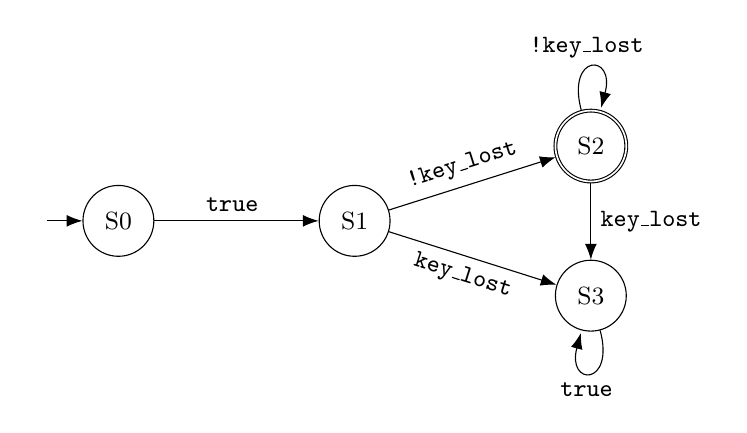
\begin{tikzpicture}[>={Latex[length=2mm]}, initial text=, font=\small, every state/.style={minimum size=9mm, inner sep=1pt}]
            \node[state, initial] (S0) at (0.00,0.00) {S0};
\node[state] (S1) at (3.00,0.00) {S1};
\node[state, accepting] (S2) at (6.00,0.95) {S2};
\node[state] (S3) at (6.00,-0.95) {S3};
\path[->] (S0) edge node[above, sloped, align=center, font=\small] {\texttt{true}} (S1);
\path[->] (S1) edge node[above, sloped, align=center, font=\small] {\texttt{!key\_lost}} (S2);
\path[->] (S1) edge node[below, sloped, align=center, font=\small] {\texttt{key\_lost}} (S3);
\path[->] (S2) edge[loop above] node[above, align=center] {\texttt{!key\_lost}} ();
\path[->] (S2) edge node[right, align=center, font=\small] {\texttt{key\_lost}} (S3);
\path[->] (S3) edge[loop below] node[below, align=center] {\texttt{true}} ();

        \end{tikzpicture}
        \caption{Raw MONA automaton, with state S0.}
        \label{fig:mona-pre}
    \end{subfigure}

    \bigskip
    \begin{subfigure}{\textwidth}
        \centering
        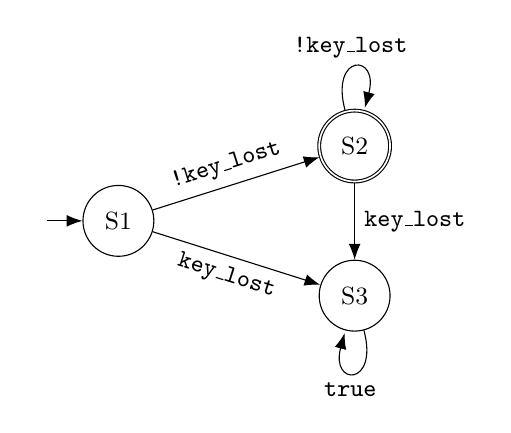
\begin{tikzpicture}[>={Latex[length=2mm]}, initial text=, font=\small, every state/.style={minimum size=9mm, inner sep=1pt}]
            \node[state, initial] (S1) at (0.00,0.00) {S1};
\node[state, accepting] (S2) at (3.00,0.95) {S2};
\node[state] (S3) at (3.00,-0.95) {S3};
\path[->] (S1) edge node[above, sloped, align=center, font=\small] {\texttt{!key\_lost}} (S2);
\path[->] (S1) edge node[below, sloped, align=center, font=\small] {\texttt{key\_lost}} (S3);
\path[->] (S2) edge[loop above] node[above, align=center] {\texttt{!key\_lost}} ();
\path[->] (S2) edge node[right, align=center, font=\small] {\texttt{key\_lost}} (S3);
\path[->] (S3) edge[loop below] node[below, align=center] {\texttt{true}} ();

        \end{tikzpicture}
        \caption{After the FL-AT fork removes state S0.}
        \label{fig:mona-post1}
    \end{subfigure}

    \bigskip
    \begin{subfigure}{\textwidth}
        \centering
        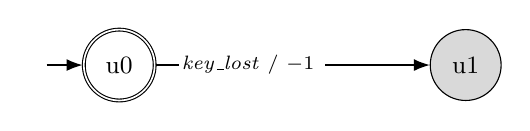
\begin{tikzpicture}[>={Latex[length=2mm]}, initial text=, font=\small, every state/.style={minimum size=9mm, inner sep=1pt}]
            \node[state, initial, accepting] (u0) at (0.00,0.00) {u0};
\node[state, fill=gray!30] (u1) at (4.40,0.00) {u1};
\path[->] (u0) edge[] node[pos=0.35, align=center, font=\scriptsize, fill=white, inner sep=1pt] {$\mathit{key\_lost}$ / $-1$} (u1);

        \end{tikzpicture}
        \caption{After the post-process merges the ``no step yet'' start into its idle twin.}
        \label{fig:mona-post2}
    \end{subfigure}
    \caption{The automaton of Absence(\texttt{key\_lost}) before and after the two removals of redundant states.}
    \label{fig:mona-stages}
\end{figure}

Listing~\ref{lst:mona-rm} gives the text of the machine in panel~(c). The implicit stay of u0 is not listed, and there are no pending promises, since the only promise is hard and its violation leads to the well.

\lstinputlisting[caption={The Reward Machine of the hard clause Absence(\texttt{key\_lost}).},label={lst:mona-rm}]{images/farm/mona.rm.txt}

%%%%%%%%%%%%%%%%%%%%%%%%%%%%%%%%%%%%%%%%%%%%%%%%%%%%%%%%%%%%%%%%%%%%%%%%%%%%%%%
%                               RUNNING EXAMPLES                              %
%%%%%%%%%%%%%%%%%%%%%%%%%%%%%%%%%%%%%%%%%%%%%%%%%%%%%%%%%%%%%%%%%%%%%%%%%%%%%%%

\chapter{Running examples}
\label{app:running}
\raggedbottom
% The brief asks for these machines in the ``Formatting examples'' appendix. That appendix is the LaTeX style sample marked for removal, so they sit here to survive its removal; move them if preferred.
Each section gives the natural-language task, the clauses and LTLf formulas the pipeline produced, the text of the Reward Machine and its graph, for the DoorKey environment. The texts and graphs are the unedited outputs of the runs described in Section~\ref{sec:examples-produced}, and the formulas are written in standard notation. All Reward Machine graphs of the thesis, including panel~(c) of Figure~\ref{fig:mona-stages}, follow one convention. States run from left to right in the order of progress. An arrow without a source marks the initial state, a double circle a final or accepting state and a grey circle the rejecting well. An edge draws all the transitions between two states and is labelled \textit{guard / reward}, where $\neg$ stands for \texttt{!} and $\land$ for \texttt{\&}. An edge with more than two guards shows only their number and their reward, for instance \textit{4 guards, $-1$}, and the listing has the conditions. Implicit stays are not drawn: when no transition of a state matches the event, the machine stays in the state and pays the default reward.

\section{Example 1: a sequence}
\label{app:ex1}
\textbf{Task.} Pick up the key, then open the door, then reach the goal.

\noindent{\footnotesize
\begin{tabularx}{\textwidth}{@{}>{\raggedright\arraybackslash}p{3.3cm}>{\raggedright\arraybackslash}p{4.3cm}l>{\raggedright\arraybackslash}X@{}}
\toprule
\textbf{Clause} & \textbf{Template} & \textbf{Priority} & \textbf{LTLf} \\ \midrule
Pick up the key & Existence(\texttt{has\_key}) & hard & $\mathrm{F}\,\mathit{has\_key}$ \\
Do not open the door before picking up the key & Precedence(\texttt{has\_key}, \texttt{door\_open}) & hard & $(\neg\mathit{door\_open}\ \mathrm{U}\ \mathit{has\_key}) \lor \mathrm{G}\,\neg\mathit{door\_open}$ \\
Open the door & Existence(\texttt{door\_open}) & hard & $\mathrm{F}\,\mathit{door\_open}$ \\
Do not reach the goal before opening the door & Precedence(\texttt{door\_open}, \texttt{at\_goal}) & hard & $(\neg\mathit{at\_goal}\ \mathrm{U}\ \mathit{door\_open}) \lor \mathrm{G}\,\neg\mathit{at\_goal}$ \\
Reach the goal & Existence(\texttt{at\_goal}) & hard & $\mathrm{F}\,\mathit{at\_goal}$ \\ \bottomrule
\end{tabularx}}

The machine is Listing~\ref{lst:farm-example1} and its graph Figure~\ref{fig:ex1-rm}. State u1 is reached after the key, u3 after the key and the door, and u4, the final state, after the goal. Any event out of order, such as opening the door without the key or reaching the goal too early, leads to the well u2 with reward $-1$. Progress pays 0.1 or 0.2, and the goal pays 1.1 to 1.3: the 1 of the final state plus the progress of the step.

\begin{figure}[H]
\centering
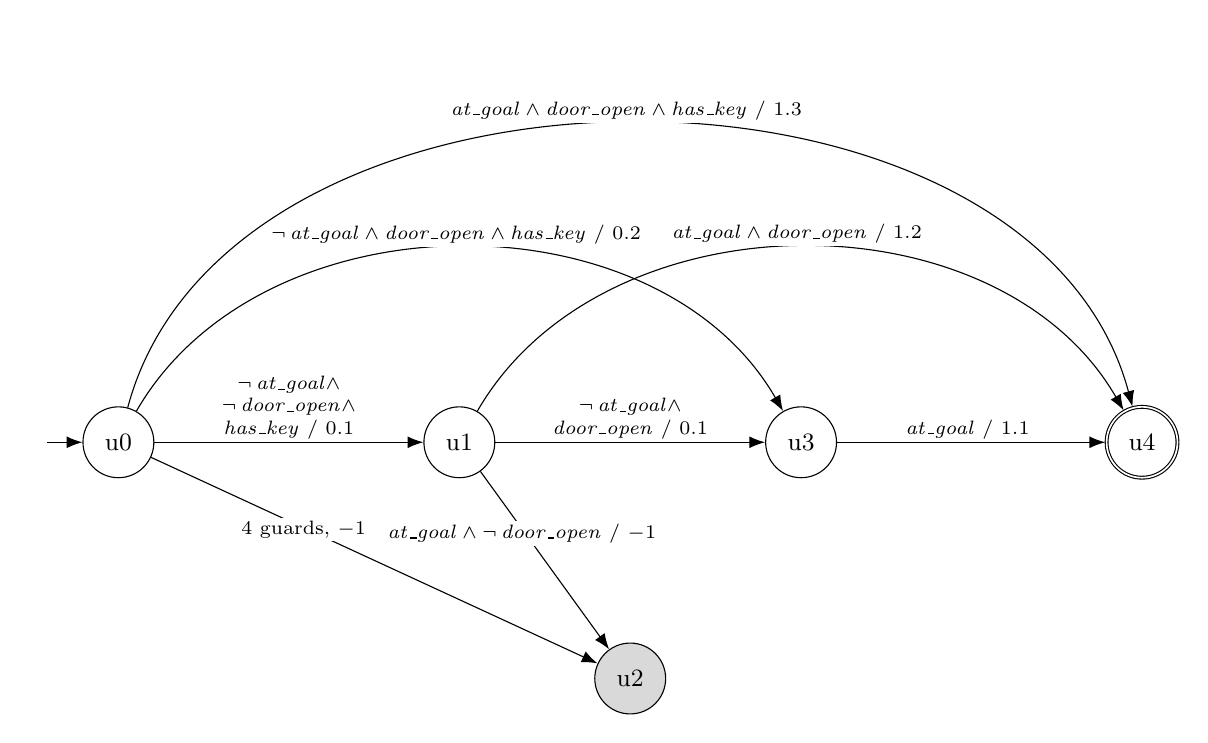
\begin{tikzpicture}[>={Latex[length=2mm]}, initial text=, font=\small, every state/.style={minimum size=9mm, inner sep=1pt}]
\node[state, initial] (u0) at (0.00,0.00) {u0};
\node[state] (u1) at (4.33,0.00) {u1};
\node[state, fill=gray!30] (u2) at (6.50,-3.00) {u2};
\node[state] (u3) at (8.67,0.00) {u3};
\node[state, accepting] (u4) at (13.00,0.00) {u4};
\path[->] (u0) edge[] node[above, align=center, font=\scriptsize, fill=white, inner sep=1pt] {$\neg\,\mathit{at\_goal} \land$ \\ $\neg\,\mathit{door\_open} \land$ \\ $\mathit{has\_key}$ / $0.1$} (u1);
\path[->] (u0) edge[] node[pos=0.35, align=center, font=\scriptsize, fill=white, inner sep=1pt] {4 guards, $-1$} (u2);
\path[->] (u0) edge[out=60, in=120] node[above, align=center, font=\scriptsize, fill=white, inner sep=1pt] {$\neg\,\mathit{at\_goal} \land \mathit{door\_open} \land \mathit{has\_key}$ / $0.2$} (u3);
\path[->] (u0) edge[out=75, in=105] node[above, align=center, font=\scriptsize, fill=white, inner sep=1pt] {$\mathit{at\_goal} \land \mathit{door\_open} \land \mathit{has\_key}$ / $1.3$} (u4);
\path[->] (u1) edge[] node[above, align=center, font=\scriptsize, fill=white, inner sep=1pt] {$\neg\,\mathit{at\_goal} \land$ \\ $\mathit{door\_open}$ / $0.1$} (u3);
\path[->] (u1) edge[] node[pos=0.35, align=center, font=\scriptsize, fill=white, inner sep=1pt] {$\mathit{at\_goal} \land \neg\,\mathit{door\_open}$ / $-1$} (u2);
\path[->] (u1) edge[out=60, in=120] node[above, align=center, font=\scriptsize, fill=white, inner sep=1pt] {$\mathit{at\_goal} \land \mathit{door\_open}$ / $1.2$} (u4);
\path[->] (u3) edge[] node[above, align=center, font=\scriptsize, fill=white, inner sep=1pt] {$\mathit{at\_goal}$ / $1.1$} (u4);

\end{tikzpicture}
\caption{The graph of the Reward Machine of example 1.}
\label{fig:ex1-rm}
\end{figure}

\section{Example 2: a hard rule}
\label{app:ex2}
\textbf{Task.} Reach the goal, and if you drop the key, pick it up right away.

\noindent{\footnotesize
\begin{tabularx}{\textwidth}{@{}>{\raggedright\arraybackslash}p{3.3cm}>{\raggedright\arraybackslash}p{4.3cm}l>{\raggedright\arraybackslash}X@{}}
\toprule
\textbf{Clause} & \textbf{Template} & \textbf{Priority} & \textbf{LTLf} \\ \midrule
reach the goal & Existence(\texttt{at\_goal}) & hard & $\mathrm{F}\,\mathit{at\_goal}$ \\
if the key is dropped, pick it up right away & ChainResponse(\texttt{key\_lost}, \texttt{has\_key}) & hard & $\mathrm{G}\,(\mathit{key\_lost} \rightarrow \mathrm{X}\,\mathit{has\_key})$ \\ \bottomrule
\end{tabularx}}

Listing~\ref{lst:ex2-rm} gives the machine and Figure~\ref{fig:ex2-rm} its graph. State u1 means that the key was dropped and putting it back is pending, and u3 that the goal was reached with that promise still open. The well u4 is entered with reward $-1$ when the key is not back at the next step. The final state u2 pays 1.2 when the goal is reached with the key in hand and 1.1 when the repair comes after the goal.

\lstinputlisting[caption={The Reward Machine of example 2.},label={lst:ex2-rm}]{images/farm/rm-ex2.txt}

\begin{figure}[H]
\centering
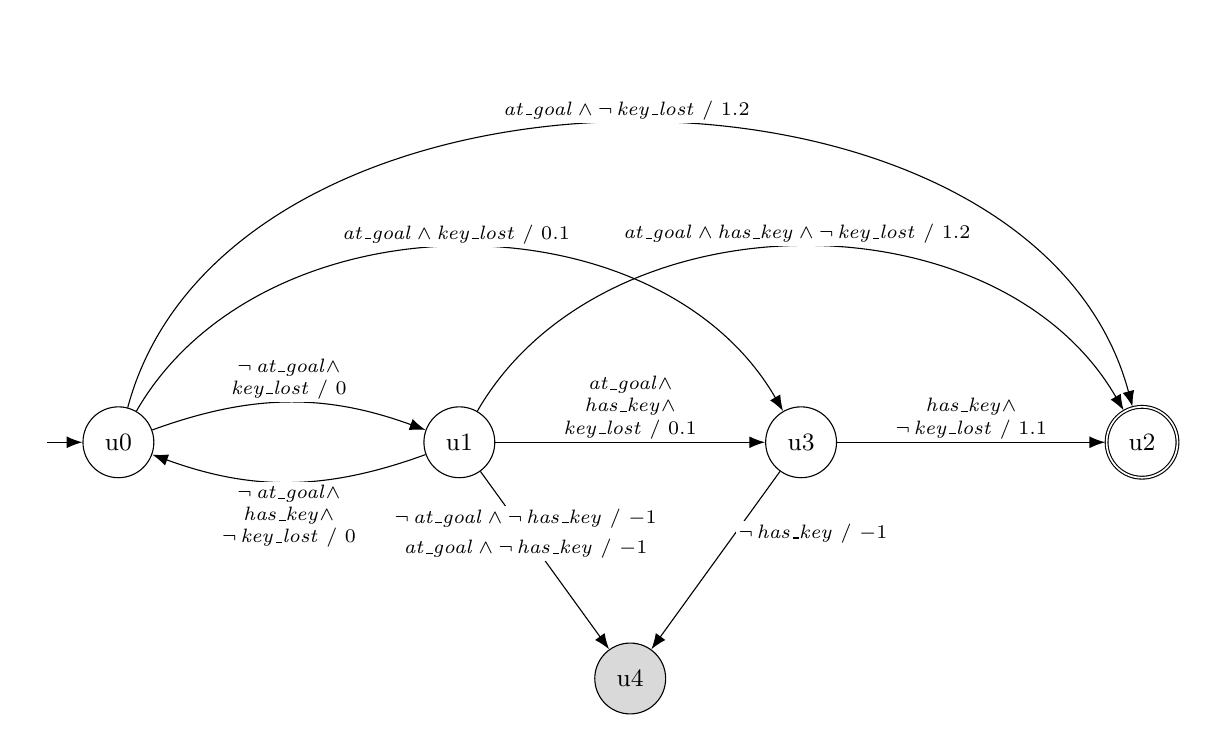
\begin{tikzpicture}[>={Latex[length=2mm]}, initial text=, font=\small, every state/.style={minimum size=9mm, inner sep=1pt}]
\node[state, initial] (u0) at (0.00,0.00) {u0};
\node[state] (u1) at (4.33,0.00) {u1};
\node[state, accepting] (u2) at (13.00,0.00) {u2};
\node[state] (u3) at (8.67,0.00) {u3};
\node[state, fill=gray!30] (u4) at (6.50,-3.00) {u4};
\path[->] (u0) edge[bend left=20] node[above, align=center, font=\scriptsize, fill=white, inner sep=1pt] {$\neg\,\mathit{at\_goal} \land$ \\ $\mathit{key\_lost}$ / $0$} (u1);
\path[->] (u0) edge[out=75, in=105] node[above, align=center, font=\scriptsize, fill=white, inner sep=1pt] {$\mathit{at\_goal} \land \neg\,\mathit{key\_lost}$ / $1.2$} (u2);
\path[->] (u0) edge[out=60, in=120] node[above, align=center, font=\scriptsize, fill=white, inner sep=1pt] {$\mathit{at\_goal} \land \mathit{key\_lost}$ / $0.1$} (u3);
\path[->] (u1) edge[] node[pos=0.35, align=center, font=\scriptsize, fill=white, inner sep=1pt] {$\neg\,\mathit{at\_goal} \land \neg\,\mathit{has\_key}$ / $-1$ \\[3pt] $\mathit{at\_goal} \land \neg\,\mathit{has\_key}$ / $-1$} (u4);
\path[->] (u1) edge[bend left=20] node[below, align=center, font=\scriptsize, fill=white, inner sep=1pt] {$\neg\,\mathit{at\_goal} \land$ \\ $\mathit{has\_key} \land$ \\ $\neg\,\mathit{key\_lost}$ / $0$} (u0);
\path[->] (u1) edge[out=60, in=120] node[above, align=center, font=\scriptsize, fill=white, inner sep=1pt] {$\mathit{at\_goal} \land \mathit{has\_key} \land \neg\,\mathit{key\_lost}$ / $1.2$} (u2);
\path[->] (u1) edge[] node[above, align=center, font=\scriptsize, fill=white, inner sep=1pt] {$\mathit{at\_goal} \land$ \\ $\mathit{has\_key} \land$ \\ $\mathit{key\_lost}$ / $0.1$} (u3);
\path[->] (u3) edge[] node[pos=0.35, right, align=center, font=\scriptsize, fill=white, inner sep=1pt] {$\neg\,\mathit{has\_key}$ / $-1$} (u4);
\path[->] (u3) edge[] node[above, align=center, font=\scriptsize, fill=white, inner sep=1pt] {$\mathit{has\_key} \land$ \\ $\neg\,\mathit{key\_lost}$ / $1.1$} (u2);

\end{tikzpicture}
\caption{The graph of the Reward Machine of example 2.}
\label{fig:ex2-rm}
\end{figure}

\section{Example 3: a soft preference}
\label{app:ex3}
\textbf{Task.} Reach the goal, ideally without ever losing the key.

\noindent{\footnotesize
\begin{tabularx}{\textwidth}{@{}>{\raggedright\arraybackslash}p{3.3cm}>{\raggedright\arraybackslash}p{4.3cm}l>{\raggedright\arraybackslash}X@{}}
\toprule
\textbf{Clause} & \textbf{Template} & \textbf{Priority} & \textbf{LTLf} \\ \midrule
reach the goal & Existence(\texttt{at\_goal}) & hard & $\mathrm{F}\,\mathit{at\_goal}$ \\
never lose the key & Absence(\texttt{key\_lost}) & soft & $\neg\,\mathrm{F}\,\mathit{key\_lost}$ \\ \bottomrule
\end{tabularx}}

Listing~\ref{lst:ex3-rm} gives the machine and Figure~\ref{fig:ex3-rm} its graph. Only the goal is hard, so the machine has no well. Losing the key costs $-0.5$ and moves the machine to u1. It returns to u0 at the next step without a loss, so each new loss is charged again, as Section~\ref{sec:step4} describes for soft rules. The goal pays 1.1, or 0.6 when the loss happens in the very step of the goal.

\lstinputlisting[caption={The Reward Machine of example 3.},label={lst:ex3-rm}]{images/farm/rm-ex3.txt}

\begin{figure}[H]
\centering
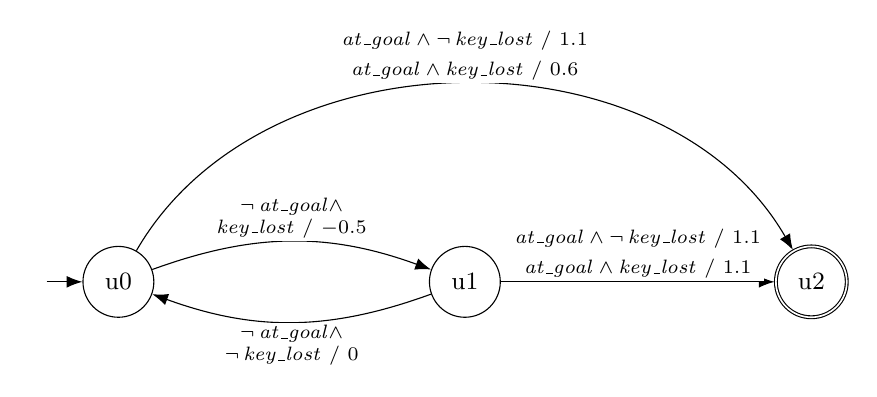
\begin{tikzpicture}[>={Latex[length=2mm]}, initial text=, font=\small, every state/.style={minimum size=9mm, inner sep=1pt}]
\node[state, initial] (u0) at (0.00,0.00) {u0};
\node[state] (u1) at (4.40,0.00) {u1};
\node[state, accepting] (u2) at (8.80,0.00) {u2};
\path[->] (u0) edge[bend left=20] node[above, align=center, font=\scriptsize, fill=white, inner sep=1pt] {$\neg\,\mathit{at\_goal} \land$ \\ $\mathit{key\_lost}$ / $-0.5$} (u1);
\path[->] (u0) edge[out=60, in=120] node[above, align=center, font=\scriptsize, fill=white, inner sep=1pt] {$\mathit{at\_goal} \land \neg\,\mathit{key\_lost}$ / $1.1$ \\[3pt] $\mathit{at\_goal} \land \mathit{key\_lost}$ / $0.6$} (u2);
\path[->] (u1) edge[bend left=20] node[below, align=center, font=\scriptsize, fill=white, inner sep=1pt] {$\neg\,\mathit{at\_goal} \land$ \\ $\neg\,\mathit{key\_lost}$ / $0$} (u0);
\path[->] (u1) edge[] node[above, align=center, font=\scriptsize, fill=white, inner sep=1pt] {$\mathit{at\_goal} \land \neg\,\mathit{key\_lost}$ / $1.1$ \\[3pt] $\mathit{at\_goal} \land \mathit{key\_lost}$ / $1.1$} (u2);

\end{tikzpicture}
\caption{The graph of the Reward Machine of example 3.}
\label{fig:ex3-rm}
\end{figure}

\section{Example 4: a task made only of rules}
\label{app:ex4}
\textbf{Task.} If you drop the key, pick it up again.

\noindent{\footnotesize
\begin{tabularx}{\textwidth}{@{}>{\raggedright\arraybackslash}p{3.3cm}>{\raggedright\arraybackslash}p{4.3cm}l>{\raggedright\arraybackslash}X@{}}
\toprule
\textbf{Clause} & \textbf{Template} & \textbf{Priority} & \textbf{LTLf} \\ \midrule
Response(\texttt{key\_lost}, \texttt{has\_key}) & Response(\texttt{key\_lost}, \texttt{has\_key}) & hard & $\mathrm{G}\,(\mathit{key\_lost} \rightarrow \mathrm{F}\,\mathit{has\_key})$ \\ \bottomrule
\end{tabularx}}

The only clause is a rule, so the machine has no goal and no final state (Listing~\ref{lst:ex4-rm} and Figure~\ref{fig:ex4-rm}). State u0 is accepting: nothing is owed there. State u1 owes the key, and \texttt{PENDING\_\allowbreak PROMISES} lists it with one hard promise. If the environment ends the episode in u1, the machine charges $-1$ once, the value \texttt{HARD\_\allowbreak FAILED\_\allowbreak REWARD}. In u0 it charges nothing. Dropping the key costs $-0.1$ and picking it up returns $+0.1$, so the two shaping rewards cancel over the cycle.

\lstinputlisting[caption={The Reward Machine of example 4, a task made only of rules.},label={lst:ex4-rm}]{images/farm/rm-ex4.txt}

\begin{figure}[H]
\centering
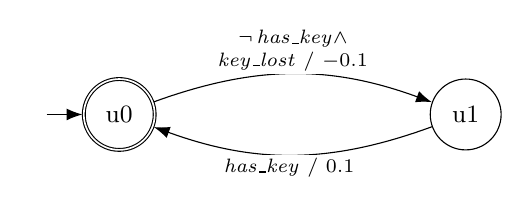
\begin{tikzpicture}[>={Latex[length=2mm]}, initial text=, font=\small, every state/.style={minimum size=9mm, inner sep=1pt}]
\node[state, initial, accepting] (u0) at (0.00,0.00) {u0};
\node[state] (u1) at (4.40,0.00) {u1};
\path[->] (u0) edge[bend left=20] node[above, align=center, font=\scriptsize, fill=white, inner sep=1pt] {$\neg\,\mathit{has\_key} \land$ \\ $\mathit{key\_lost}$ / $-0.1$} (u1);
\path[->] (u1) edge[bend left=20] node[below, align=center, font=\scriptsize, fill=white, inner sep=1pt] {$\mathit{has\_key}$ / $0.1$} (u0);

\end{tikzpicture}
\caption{The graph of the Reward Machine of example 4.}
\label{fig:ex4-rm}
\end{figure}
\flushbottom

%%%%%%%%%%%%%%%%%%%%%%%%%%%%%%%%%%%%%%%%%%%%%%%%%%%%%%%%%%%%%%%%%%%%%%%%%%%%%%%
%                             FORMATTING EXAMPLES                             %
%%%%%%%%%%%%%%%%%%%%%%%%%%%%%%%%%%%%%%%%%%%%%%%%%%%%%%%%%%%%%%%%%%%%%%%%%%%%%%%

\chapter{Formatting examples}
\label{app:examples}
This appendix collects formatting examples for figures, tables, plots and algorithms. It will be removed before submission.

Figure~\ref{fig:example-single} shows a single image.

\begin{figure}[H]
    \centering
    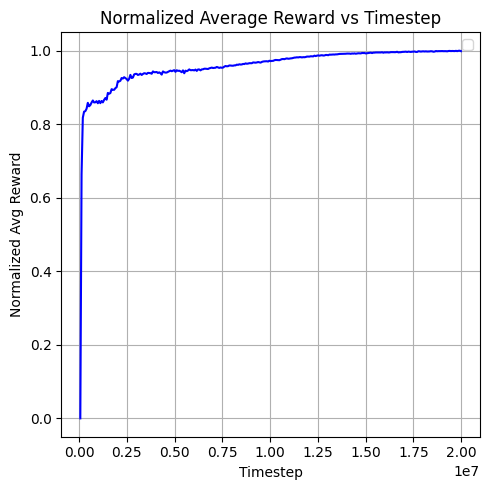
\includegraphics[width=0.5\linewidth]{images/spread_1.png}
    \caption{Example of a single image.}
    \label{fig:example-single}
\end{figure}

Figure~\ref{fig:example-subfigures} shows two subfigures side by side, Figures~\ref{fig:example-subfig-a} and~\ref{fig:example-subfig-b}.

\begin{figure}[H]
    \centering
    \begin{subfigure}{0.45\textwidth}
        \centering
        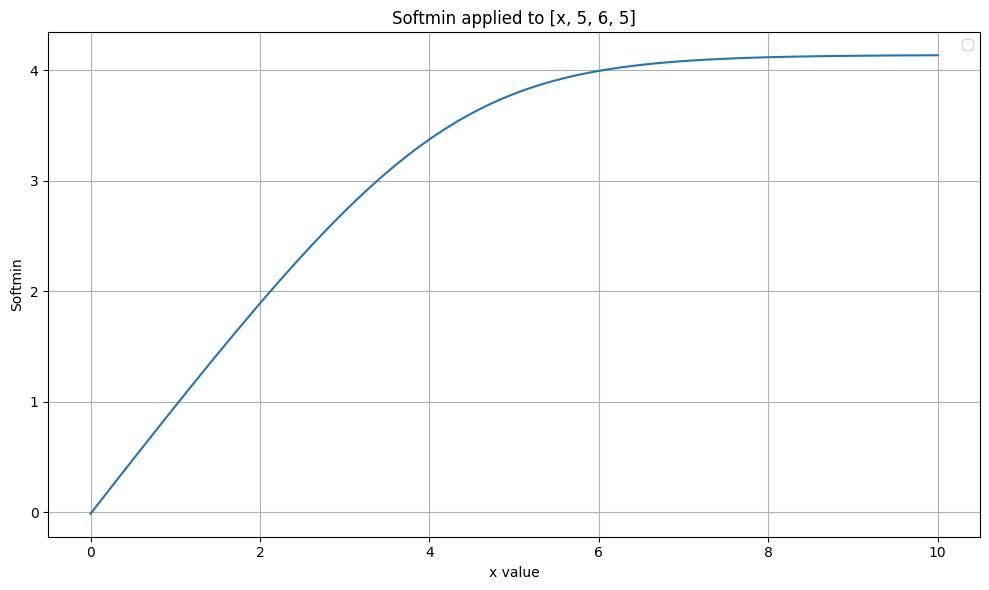
\includegraphics[width=\linewidth]{images/softmin_one.png}
        \caption{First subfigure.}
        \label{fig:example-subfig-a}
    \end{subfigure}
    \hfill
    \begin{subfigure}{0.45\textwidth}
        \centering
        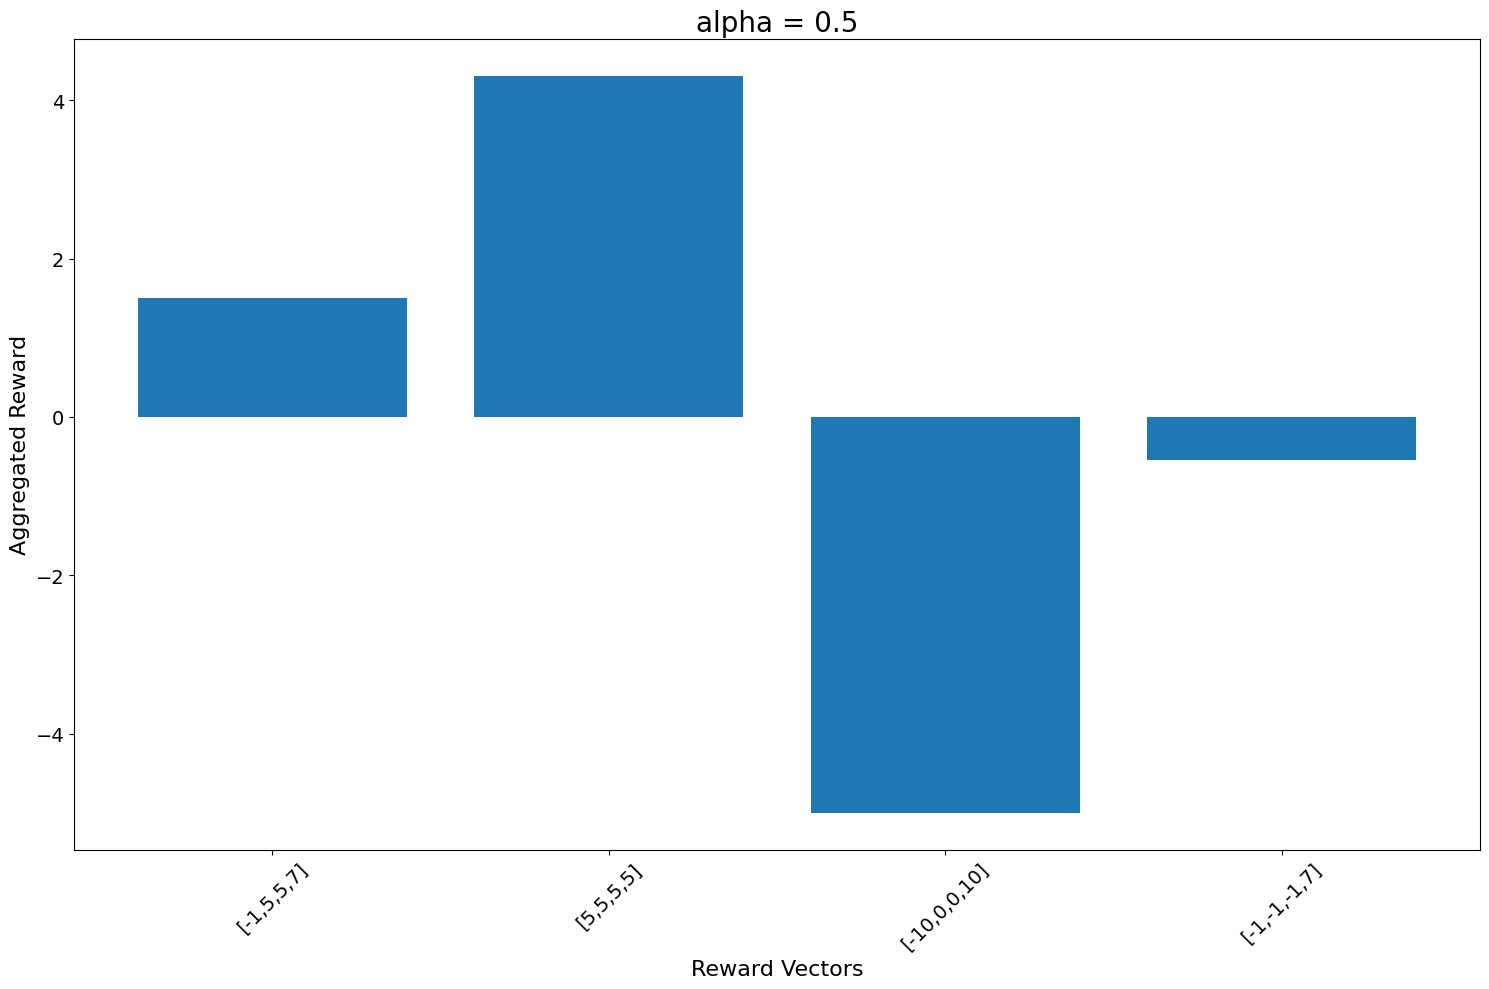
\includegraphics[width=\linewidth]{images/softminmean_one.png}
        \caption{Second subfigure.}
        \label{fig:example-subfig-b}
    \end{subfigure}
    \caption{Example of two subfigures side by side.}
    \label{fig:example-subfigures}
\end{figure}

Figure~\ref{fig:example-tikz} shows a diagram drawn with TikZ.

\begin{figure}[H]
    \centering
    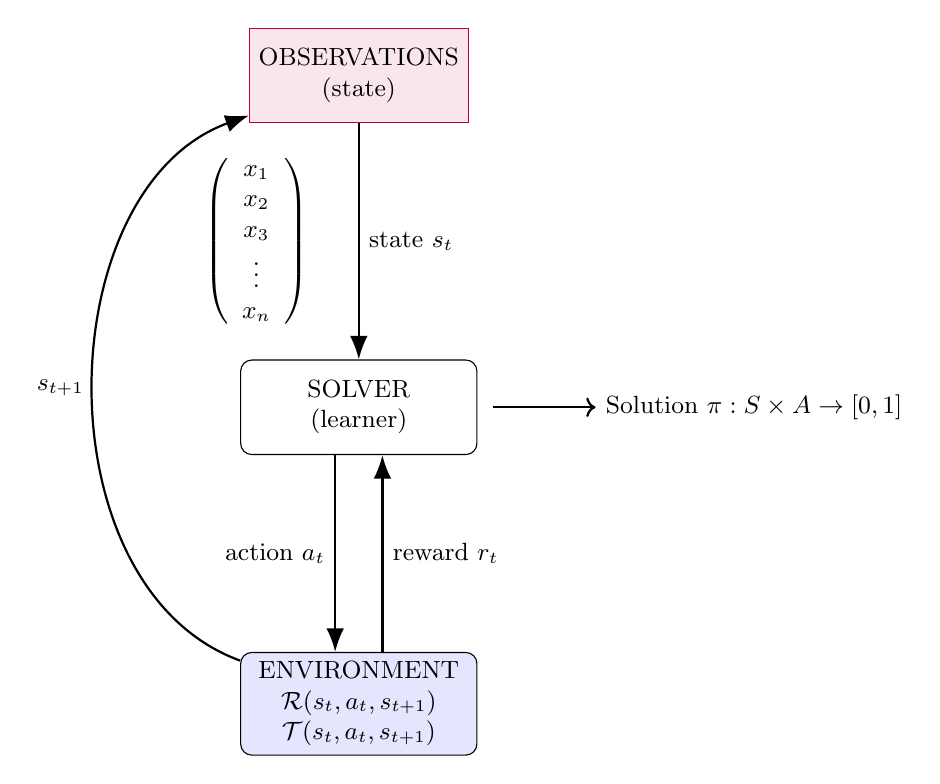
\begin{tikzpicture}[
        font=\small,
        box/.style={draw, rounded corners, minimum width=3cm, minimum height=1.2cm, align=center},
        arrow/.style={-{Latex[length=3mm]}, thick},
        obs/.style={draw=purple, fill=purple!10, minimum width=2.5cm, minimum height=1.2cm, align=center}
    ]

    % Nodes
    \node[obs] (obs) {OBSERVATIONS\\(state)};
    \node[box, below=3cm of obs] (solver) {SOLVER\\(learner)};
    \node[box, below=2.5cm of solver, fill=blue!10] (env) {ENVIRONMENT\\$\mathcal{R}(s_t, a_t, s_{t+1})$\\$\mathcal{T}(s_t, a_t, s_{t+1})$};

    % Vector colocated near observation → solver arrow
    \node at ($(obs)!0.5!(solver) + (-1.3,0)$) (vec) {$\left(\begin{array}{c}
    x_1 \\ x_2 \\ x_3 \\ \vdots \\ x_n
    \end{array}\right)$};

    % Policy notation (replaces "solution")
    \draw[->, thick] (solver.east) ++(0.2,0) -- ++(1.3,0) node[right] {Solution $\pi : S \times A \rightarrow [0, 1]$};

    % Arrows
    \draw[arrow] (obs) -- node[right] {state $s_t$} (solver);
    \draw[arrow] ([xshift=-0.3cm]solver.south) -- ([xshift=-0.3cm]env.north) node[midway, left] {action $a_t$};
    \draw[arrow] ([xshift=0.3cm]env.north) -- ([xshift=0.3cm]solver.south) node[midway, right] {reward $r_t$};
    \draw[arrow] (env) to[out=160, in=-160] node[left] {$s_{t+1}$} (obs);

    \end{tikzpicture}
    \caption{Example of a TikZ diagram.}
    \label{fig:example-tikz}
\end{figure}

Figure~\ref{fig:example-plot} shows a multi-panel plot drawn with \texttt{pgfplots}.

\begin{figure}[H]
    \centering
    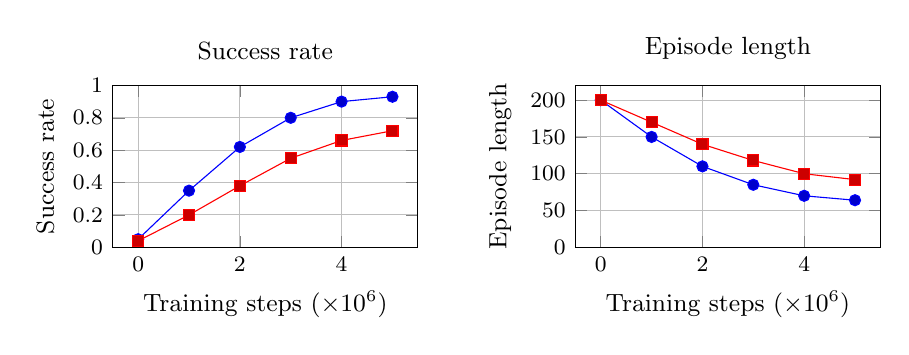
\begin{tikzpicture}
        \begin{groupplot}[
            group style={group size=2 by 1, horizontal sep=2cm},
            width=0.45\linewidth,
            height=0.3\linewidth,
            xlabel={Training steps ($\times 10^{6}$)},
            grid=major,
            tick label style={font=\footnotesize},
            label style={font=\small},
            title style={font=\small},
            legend style={font=\footnotesize}
        ]
            \nextgroupplot[title={Success rate}, ylabel={Success rate}, ymin=0, ymax=1,
                legend to name=grouplegend, legend columns=2]
                \addplot coordinates {(0,0.05) (1,0.35) (2,0.62) (3,0.80) (4,0.90) (5,0.93)};
                \addlegendentry{Series A}
                \addplot coordinates {(0,0.04) (1,0.20) (2,0.38) (3,0.55) (4,0.66) (5,0.72)};
                \addlegendentry{Series B}
            \nextgroupplot[title={Episode length}, ylabel={Episode length}, ymin=0]
                \addplot coordinates {(0,200) (1,150) (2,110) (3,85) (4,70) (5,64)};
                \addplot coordinates {(0,200) (1,170) (2,140) (3,118) (4,100) (5,92)};
        \end{groupplot}
    \end{tikzpicture}

    \ref{grouplegend}
    \caption[Example of a two-panel plot with illustrative data]{Example of a two-panel plot with illustrative data: success rate and episode length against training steps for two series.}
    \label{fig:example-plot}
\end{figure}

Table~\ref{tab:example-booktabs} shows a table in \texttt{booktabs} format.

\begin{table}[H]
\centering
\caption{Example of a \texttt{booktabs} table with illustrative data.}
\label{tab:example-booktabs}
\renewcommand{\arraystretch}{1.2}
\begin{tabular}{@{}lrr@{}}
\toprule
\textbf{Series} & \textbf{Success rate} & \textbf{Episode length} \\ \midrule
Series A        & 0.93                  & 64                      \\
Series B        & 0.72                  & 92                      \\ \bottomrule
\end{tabular}
\end{table}

Algorithm~\ref{alg:example-pseudocode} shows a block of pseudocode.

\begin{algorithm}[H]
\caption{Example of a pseudocode block}
\textbf{Input:} list of items $L$, threshold $\theta$ \\
\textbf{Output:} list of kept items $L'$
\begin{algorithmic}[1]
\Procedure{Filter}{$L, \theta$}
    \State $L' \gets \emptyset$
    \For{each $x \in L$}
        \If{$f(x) > \theta$}
            \State $L' \gets L' \cup \{x\}$ \Comment{keep the item}
        \Else
            \State \textbf{continue} \Comment{skip the item}
        \EndIf
    \EndFor
    \State \Return $L'$
\EndProcedure
\end{algorithmic}
\label{alg:example-pseudocode}
\end{algorithm}

%%%%%%%%%%%%%%%%%%%%%%%%%%%%%%%%%%%%%%%%%%%%%%%%%%%%%%%%%%%%%%%%%%%%%%%%%%%%%%%
%                               FI DEL DOCUMENT                               %
%%%%%%%%%%%%%%%%%%%%%%%%%%%%%%%%%%%%%%%%%%%%%%%%%%%%%%%%%%%%%%%%%%%%%%%%%%%%%%%

\end{document}